\documentclass[russian,utf8,simple,emptystyle]{eskdtext}
\usepackage[numberright]{eskdplain}
\usepackage{paratype}
\usepackage{longtable}
\usepackage{array}
\usepackage{epstopdf}
\usepackage{multirow}
\usepackage{amssymb,amsmath,amsthm,latexsym}
\usepackage{slashbox}
\usepackage{multirow}

\ESKDdepartment{ФЕДЕРАЛЬНОЕ АГЕНТСТВО ПО ОБРАЗОВАНИЮ РФ}
\ESKDcompany{МГТУ им. Н.Э.Баумана}
\ESKDclassCode{40 1350}
\ESKDtitle{База данных}
\ESKDdocName{<<ИС о случаях нападения акул на человека>>}
\ESKDsignature{Вариант №8}
\ESKDauthor{Гуща~А.~В}
\ESKDchecker{Ревунков~Г.~И}
\ESKDtitleApprovedBy{\hspace{0cm}}{Ревунков~Г.~И}
\ESKDtitleAgreedBy{\hspace{0cm}}{Ревунков~Г.~И}
\ESKDtitleDesignedBy{Студент 3 курса группы ИУ5-62}{Гуща~А.~В}

\renewcommand{\ESKDtheTitleFieldX}{%
Москва
 
\ESKDtheYear~г.}

\renewcommand{\baselinestretch}{1}
\renewcommand{\arraystretch}{1.5}

\usepackage{listings}
\usepackage{color}

\definecolor{mygreen}{rgb}{0,0.6,0}
\definecolor{mygray}{rgb}{0.5,0.5,0.5}
\definecolor{mymauve}{rgb}{0.58,0,0.82}

\lstset{ %
  backgroundcolor=\color{white},   % choose the background color; you must add \usepackage{color} or \usepackage{xcolor}
  basicstyle=\footnotesize,        % the size of the fonts that are used for the code
  breakatwhitespace=true,         % sets if automatic breaks should only happen at whitespace
  breaklines=true,                 % sets automatic line breaking
  captionpos=b,                    % sets the caption-position to bottom
  commentstyle=\color{mygreen},    % comment style
  deletekeywords={...},            % if you want to delete keywords from the given language
  escapeinside={\%*}{*)},          % if you want to add LaTeX within your code
  extendedchars=true,              % lets you use non-ASCII characters; for 8-bits encodings only, does not work with UTF-8
  frame=left,                    % adds a frame around the code
  keywordstyle=\color{blue},       % keyword style
  language=C,                 % the language of the code
  morekeywords={*,...},            % if you want to add more keywords to the set
  numbers=left,                    % where to put the line-numbers; possible values are (none, left, right)
  numbersep=5pt,                   % how far the line-numbers are from the code
  numberstyle=\tiny\color{mygray}, % the style that is used for the line-numbers
  rulecolor=\color{black},         % if not set, the frame-color may be changed on line-breaks within not-black text (e.g. comments (green here))
  showspaces=false,                % show spaces everywhere adding particular underscores; it overrides 'showstringspaces'
  showstringspaces=false,          % underline spaces within strings only
  showtabs=false,                  % show tabs within strings adding particular underscores
  stepnumber=2,                    % the step between two line-numbers. If it's 1, each line will be numbered
  stringstyle=\color{mymauve},     % string literal style
  tabsize=2,                       % sets default tabsize to 2 spaces
  title=   % show the filename of files included with \lstinputlisting; also try caption instead of title
}

\begin{document}
%\maketitle
\tableofcontents
\newpage

\section{Аннотация}
Разработано программное изделие, автоматизирующее процесс сбора и обработки статистики о случаях нападения акул на человека. Изделие представляет собой базу данных, под управлением СУБД PostgreSQL. Для упрощения работы пользователя с базой данных, было разработано графическое приложение на системе проектирования визуальных интерфейсов GtkD и мультиплатформенном системном языке программирования D.
\clearpage

\section{Введение}
С помощью системы управления базами данных (СУБД) PostgreSQL 9.2, библиотеки для разработки графический интерфейсов GtkD и языка программирования D, в рамках курсового проекта по курсу "Базы данных" создана программная система <<ИС о случаях нападения акул на человека>>. Таблицы с набором данных реализованы с помощью языка запросов SQL в СУБД PostgreSQL, а формы входных и выходных документов реализованы с помощью библиотеки GtkD и языка программирования D.

Основные функции базы данных <<ИС о случаях нападения акул на человека>>:
\begin{enumerate}
\item Ввод/изменение новых данных;
\item Выполнение запросов;
\item Формирование отчетов.
\end{enumerate}

Выбор перечисленных функций осуществляется с помощью главного меню, появляющегося при загрузке программы.

При создании системы необходимо было решить следующие задачи:
\begin{enumerate}
\item Обеспечение хранения данных в форме таблиц.
\item Обеспечение ввода и редактирования данных.
\item Обеспечение выдачи информации в виде отчетов на экран компьютера и их печати.
\item Обеспечение удобного пользовательского интерфейса.
\end{enumerate}

База данных <<ИС о случаях нападения акул на человека>> состоит из 8 таблиц:
\begin{itemize}
\item AttackCases
\item Reasons
\item Places
\item InformationSources
\item Victims
\item SharkSpecies
\item Property
\item Habitats
\end{itemize}

Для связей между этими таблицами используется механизм ссылочной целостности.
\clearpage

\section{Описание предметной области}
После введения в эксплуатацию системы <<ИС о случаях нападения акул на человека>> пользователи смогут получить актуальную статистику о случаях нападения акул на человека. Происходит нападение акулы на человека, через некоторое время информация о нападении попадает в официальные информационные агентства, откуда модератор базы данных собирает информацию о случаях нападения акул на человека. После введения информации в базу данных обычные пользователи могут просматривать статистику, сведения о нападениях, получать отчеты (например, опасность того или иного пляжа, шанс стать пострадавшим в определенных странах и сезонах). До введения в эксплуатацию системы <<ИС о случаях нападения акул на человека>> пользователям приходилось искать, систематизировать и делать выводы самостоятельно, поэтому введение системы в эксплуатацию экономит солидный объем времени пользователей.

Система <<ИС о случаях нападения акул на человека>> может быть использована в туристических агентствах для привлечения клиентов актуальной информацией и обеспечением защиты своих клиентов путем обеспечения высокой степени информированности о способах избегания встречи с акулами. Также система <<ИС о случаях нападения акул на человека>> может быть использована частными или государственными компаниями для отслеживания динамики случаев нападения акул на человека, что позволит производить прогнозирование опасных случаев и обеспечивать исполнительные органы (например, береговая охрана) актуальной информацией об уровне опасности в разных регионах.
\clearpage

\section{Функциональная модель предметной области}
\subsection{Графическая диаграмма DFD}
Функциональная модель предметной области в виде DFD-диаграммы приведена в Приложении №1. Внешние по отношению к системе объекты - это <<Пользователь>> и  <<Модератор>>. Пользователь запрашивает у системы необходимую ему информацию, затем на основе запроса система формирует статистику, графический отчет. Модератор производит поиск и первичную обработку информации перед занесением ее в базу данных.

\subsection{Графическая диаграмма IEF}
Функциональная модель предметной области в виде IDEF0-диаграммы приведена в Приложении №2. Рассмотрим последовательно все функциональные блоки, представленные на схеме.

\subsubsection{Сбор первичной информации}
Модератор производит регулярный поиск новой информации о случаях нападения акул на человека, проводя первичную фильтрацию данных. Недостоверная, неверная или неподтвержденная несколькими источниками информация должна быть отсеяна на этом этапе. Выходные данные функционального блока - данные о жертве, данные о акуле, данные о местности нападения и другая информация о нападении акулы на человека.

\subsubsection{Сбор информации о жертвах}
Первичный сбор информации не обеспечивает достаточного объема информации для получения статистики, поэтому модератор собирает уточненные данные о жертвах происшествия на основе данных о жертвах, полученных в предыдущем функциональном блоке. Входные данные - информация от новостных источников и отчеты служб. Выходные данные функционального блока - полная информация о жертве (род деятельности, год рождения, описание повреждений и т.д.) и причиненном ущербе.

\subsubsection{Сбор информации об акулах}
Первичный сбор информации не обеспечивает достаточного объема информации для получения статистики, поэтому модератор собирает уточненные данные об акулах, совершивших нападение из новостных источников и публичных отчетах служб. Входные данные - информация от новостных источников и отчеты служб. Выходные данные - полная информация о виде акулы и информация о дальнейшей судьбе конкретных экземпляров.

\subsubsection{Сбор информации о местности}
Первичный сбор информации не обеспечивает достаточного объема информации для получения статистики, поэтому модератор собирает уточненные данные о местности, в которой было совершено нападение. Данная информация необходима для проведения анализа опасности определенных районов и генерации соответствующих отчетов. Входные данные - информация от новостных источников и отчеты служб. Выходные данные - полная информация о местности, в которой было совершено нападение.

\subsection{Добавление записи}
После окончания сбора и уточнения всех необходимых данных модератор производит добавление новой записи в базу данных в соответствии с принятым в системе форматом данных. Входные данные - полная информация о нападении акулы. Выходные данные - запрос к базе данных на добавление новой записи.

\subsubsection{Редактирование данных}
Иногда модератор может совершить ошибку при сборе данных, или может появиться новая информация, относящаяся к уже занесенному в систему случаю нападения акулы на человека. В таких случаях модератор может произвести редактирование данных в базе данных в соответствии с принятым в системе формате данных. Входная информация - обновленная информация о случае нападения. Выходная информация - запрос к базе данных на обновление записи.

\subsubsection{Запрос информации}
Пользователь системы может запросить статистические сведения о случаях нападения акул на человека в соответствии с принятым в системе форматом данных (графические формы). Входные данные - данные из форм. Выходные данные - запрос к базе данных на получение информации из записи.

\subsubsection{Выдача данных}
СУБД под управлением операционной системы производит обработку запроса и выдачу необходимой информации. Входные данные - запрос к базе данных. Выходные данные - информация о случаях нападения акулы на человека, необходимая пользователю.

\subsubsection{Запрос отчета}
Пользователь системы может запросить генерацию заранее определенного типа отчета о случаях нападения акул на человека. Входные данные - тип отчета и данные формы, на основе которых будет произведена выборка данных. Выходные данные - запрос к базе данных.

\subsubsection{Генерация отчета}
С помощью специальной программы и СУБД под управлением операционной системой производится генерация отчета на основе запроса к базе данных, полученного на предыдущем этапе. Входные данные - запрос к базе данных. Выходные данные - отчет, готовый к показу пользователю или печати.

\subsection{Спецификационный вариант модели}
\begin{enumerate}
	\item Выполнение запроса и выдача его в форме таблицы:
	\begin{enumerate}
		\item Выполнение запроса <<Мониторинг количества жертв за период>>;
		\item Выполнение запроса <<Мониторинг причиненного ущерба за период>>;
		\item Выполнение запроса <<Мониторинг жертв в определенном регионе>>;
		\item Выполнение запроса <<Летальные исходы по виду акулы>>;
		\item Выполнение запроса <<Соотношение спровоцированных и не спровоцированных нападений за период>>.
	\end{enumerate}
	
	\item Создание отчетов и их выдача в виде готовых документов:
	\begin{enumerate}
		\item Создание отчета <<Опасность регионов>> и выдача его в форме готового документа;
		\item Создание отчета <<Группы риска по роду деятельности>> и выдача его в форме готового документа;
		\item Создание отчета <<Самые опасные виды акул>> и выдача его в форме готового документа;
		\item Создание отчета <<Динамика количества нападений за все время>> и выдача его в форме готового документа;
		\item Создание отчета <<Количество нападений в зависимости от времени суток>> и выдача его в форме готового документа;
	\end{enumerate}
	
	\item Ввод/редактирование информации о нападениях:
	\begin{enumerate}
		\item Функция <<Ввод/изменение случаев нападений>>;
		\item Функция <<Ввод/изменение видов акул>>;
		\item Функция <<Ввод/изменение ареалов обитания>>;
		\item Функция <<Ввод/изменение местностей нападения>>;
		\item Функция <<Ввод/изменение информации о жертвах>>;
		\item Функция <<Ввод/изменение информации о пострадавшем имуществе>>.
	\end{enumerate}
	
	\item Ввод/редактирование информации о новостных источниках:
	\begin{enumerate}
		\item Функция <<Ввод/изменение источников информации>>.
	\end{enumerate}
\end{enumerate}
\clearpage

\section{Структурная схема системы}
Структурная схема системы представлена в приложении №3. Автоматизированная система <<ИС о случаях нападения акул на человека>> состоит из трех взаимосвязанных модулей. Система должна реализовывать работу с таблицами, а именно ввод, редактирование и просмотр данных. Ввод данных - ввод новых данных в базу данных. Редактирование - изменение или удаление уже имеющихся данных. Просмотр - просмотр имеющихся данных с использованием различных методов их визуализации (фильтрация, сортировка). Работа с запросами подразумевает только их просмотр.
Работа с отчетами подразумевает указание параметров конкретного отчета (на основе этих данных генерируется отчет). После формирования отчета пользователь получает отчет в формате PDF, который можно отправить на принтер для печати.

\clearpage
\section{Инфологическая модель}
\subsection{Графическая диаграмма}
Инфологическая модель предметной области представлена в Приложении №4.

\subsection{Спецификационный вариант}

\begin{enumerate}
	\item Атрибуты:
	\begin{enumerate}
		\item \underline{КодНападения} - INT(4);
		\item Дата - DATE;
		\item ВремяСуток - INT(4);
		\item ОписаниеСобытий - TEXT(1000);
		\item ДальностьВидимостиВВоде - INT(4);
		\item \underline{КодИсточника} - INT(4);
		\item НазваниеИсточника - TEXT(200);
		\item ИнтернетАдрес - TEXT(1000);
		\item КопияСообщения - TEXT(10000);
		\item ОфициальностьИсточника - BOOL;
		\item \underline{КодМеста} - INT(4);
		\item НазваниеМеста - TEXT(200);
		\item Страна - TEXT(200);
		\item ОписаниеМеста - TEXT(1000);
		\item ТипМестаНападения - INT(4);
		\item \underline{КодПричины} - INT(4);
		\item НазваниеПричины - TEXT(200);
		\item ОписаниеПоведения - TEXT(1000);
		\item СпровоцированноеЛиПоведение - BOOL;
		\item \underline{КодВида} - INT(4);
		\item НазваниеВида - TEXT(200);
		\item ОписаниеВида - TEXT(1000);
		\item СредниеРазмеры - INT(4);
		\item РационПитания - TEXT(1000);
		\item Фотографии - TEXT(1000);
		\item СтепеньОпасности - INT(4);
		\item \underline{КодАреала} - INT(4);
		\item ОписаниеАреала - TEXT(1000);
		\item Площадь - INT(8);
		\item СтепеньПрисутствияЧеловека - FLOAT(4);
		\item \underline{КодЖертвы} - INT(4);
		\item ФИО - TEXT(200);
		\item ГодРождения - DATE;
		\item РодДеятельности - TEXT(200);
		\item ОписаниеПовреждений - TEXT(1000);
		\item ДальнейшаяСудьбаЖертвы - TEXT(1000);
		\item \underline{КодИмущества} - INT(4);
		\item ТипИмущества - TEXT(200);
		\item ОценкаУщерба - INT(8);
		\item ХарактерПовреждений - TEXT(200).
	\end{enumerate}
	
	\item Сущности:
	\begin{enumerate}
		\item СлучайНападенияАкулыНаЧеловека(\underline{КодНападения}, Дата, ВремяСуток, ОписаниеСобытий, ДальностьВидимостиВВоде);
		\item ИсточникИнформации(\underline{КодИсточника}, НазваниеИсточника, ИнтернетАдрес, КопияСообщения, ОфициальностьИсточника);
		\item МестоНападения(\underline{КодМеста}, НазваниеМеста, Страна, ОписаниеМеста, ТипМестаНападения);
		\item ПричинаАтаки(\underline{КодПричины}, НазваниеПричины, ОписаниеПоведения, СпровоцированноеЛиПоведение);
		\item ВидАкулы(\underline{КодВида}, НазваниеВида, ОписаниеВида, СредниеРазмеры, РационПитания, Фотографии, СтепеньОпасности);
		\item Ареал(\underline{КодАреала}, ОписаниеАреала, Площадь, СтепеньПрисутствияЧеловека);
		\item Жертва(\underline{КодЖертвы}, ФИО, ГодРождения, РодДеятельности, ОписаниеПовреждений, ДальнейшаяСудьбаЖертвы);
		\item Имущество(\underline{КодИмущества}, ТипИмущества, ОценкаУщерба,  ХарактерПовреждений).
	\end{enumerate}
	
	\item Связи между сущностями:
	\begin{enumerate}
		\item КтоОпубликовал(\underline{КодНападения}, \underline{КодИсточника}) тип 1:M от СлучайНападенияАкулыНаЧеловека к ИсточникИнформации.
		\item Где(\underline{КодНападения}, \underline{КодМеста}) тип M:1 от СлучайНападенияАкулыНаЧеловека к МестоНападения.
		\item Почему(\underline{КодНападения}, \underline{КодПричины}) тип M:M от СлучайНападенияАкулыНаЧеловека к ПричинаАтаки.
		\item КтоНапал(\underline{КодНападения}, \underline{КодВида}) тип M:M от СлучайНападенияАкулыНаЧеловека к ВидАкулы.
		\item ГдеОбитает(\underline{КодВида}, \underline{КодАреала}) тип M:M от ВидАкулы к Ареал.
		\item КтоПострадал(\underline{КодНападения}, \underline{КодЖертвы}) тип M:M от СлучайНападенияАкулыНаЧеловека к Жертва.
		\item ЧтоПострадало(\underline{КодНападения}, \underline{КодИмущества}) тип M:M от СлучайНападенияАкулыНаЧеловека к Имущество.  
	\end{enumerate}
	
	\item Связи между атрибутами сущностей:
	\begin{enumerate}
		\item Сущность СлучайНападенияАкулыНаЧеловека:
		\begin{figure}[h!]
		\centering
		\includegraphics*[width=\textwidth]{inf1}
		\end{figure}
		
		\item Сущность ИсточникИнформации:
		\begin{figure}[h!]
		\centering
		\includegraphics*[width=\textwidth]{inf2}
		\end{figure}
		\clearpage
		
		\item Сущность МестоНападения:
		\begin{figure}[h!]
		\centering
		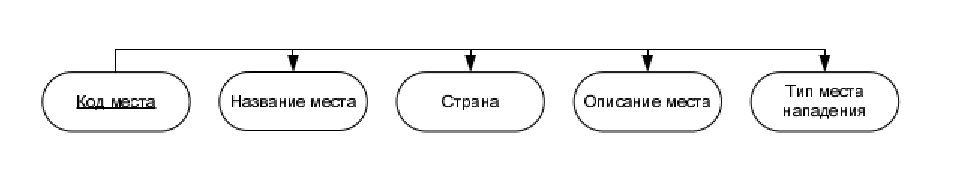
\includegraphics[width=\textwidth]{inf3}
		\end{figure}
		
		\item Сущность ПричинаАтаки:
		\begin{figure}[h!]
		\centering
		\includegraphics*[width=\textwidth]{inf4}
		\end{figure}
				
		\item Сущность Ареал:
		\begin{figure}[h!]
		\centering
		\includegraphics*[width=\textwidth]{inf5}
		\end{figure}		
		
		\item Сущность ВидАкулы:
		\begin{figure}[h!]
		\centering
		\includegraphics*[width=\textwidth]{inf6}
		\end{figure}
		
		\item Сущность Жертва:
		\begin{figure}[h!]
		\centering
		\includegraphics*[width=\textwidth]{inf7}
		\end{figure}	
		\clearpage
		
		\item Сущность Имущество:
		\begin{figure}[h!]
		\centering
		\includegraphics*[width=\textwidth]{inf8}
		\end{figure}							
	\end{enumerate}
\end{enumerate}

Из графической диаграммы инфологической модели видно, что все атрибуты всех сущностей атомарные (то есть неделимы) и не содержат повторяющихся групп. Следовательно, модель находится в первой нормальной форме.

Первичный ключ функционально и полно определяет все атрибуты, т.е. любой из атрибутов полностью зависит от первичного ключа, во всех сущностях предметной области. Следовательно, инфологическая модель нормализована ко второй нормальной форме.

Для всех сущностей все атрибуты зависят от первичного ключа и не зависят друг от друга. Таким образом, учитывая, что модель предметной области уже находится во второй нормальной форме, она нормализована и к третьей нормальной форме.

После проведенных преобразований видно, что все атрибуты зависят только от первичного ключа и отсутствуют многозначные зависимости, т.е. инфологическая модель системы находится в четвертой нормальной форме.
\clearpage

\section{Выбор СУБД}
Для реализации базы данных использована СУБД PostgreSQL. Она отвечает всем необходимым требованиям для реализации сущностей, связей между ними, запросов, требованиям безопасности и качественным требованиям. Также для базы данных сделано приложение на D и GtkD, что облегчает конечную визуализацию итоговой базы данных пользователю в виде единого независимого файла и объединяет службу генерации отчетов с интерфейсом базы данных.

\section{Датологическая модель предметной области}
\subsection{Графическая диаграмма}
Даталогическая модель предметной области, являющаяся отображением инфологической модели, представлена в Приложении №5.

\subsection{Спецификация}
\begin{center}
	\small
	\begin{longtable}{l|l|l|l}
		\caption{Таблицы в базе данных} \\
		№ & Название & Атрибут - Тип данных & Первичный ключ \\
		\hline
		1 & AttackCases & $\begin{aligned}
							& AttackCaseID &  & INT(4) \\
							& Date &  & DATE \\
							& DayTime &  & INT(4) \\
							& CaseDescr &  & TEXT \\
							& ViewDist &  & INT(4) \\
							& PlaceID &  & INT(4)
						  \end{aligned}$ & AttackCaseID \\
		\hline
		2 & InformationSources & $\begin{aligned}
							& InformationSourceID &  & INT(4) \\
							& AttackCaseID &  & INT(4) \\
							& SourceName &  & TEXT \\
							& URL &  & TEXT \\
							& MessageCopy &  & TEXT \\
							& IsOffical &  & BOOL
						  \end{aligned}$ & InformationSourceID \\		
		\hline						  
		3 & Places & $\begin{aligned}
							& PlaceID &  & INT(4) \\
							& PlaceName &  & TEXT \\
							& Country &  & TEXT \\
							& PlaceDescr &  & TEXT \\
							& PlaceType &  & INT(4)
						  \end{aligned}$ & PlaceID \\	
		\hline
		4 & Reasons & $\begin{aligned}
							& ReasonID &  & INT(4) \\
							& ReasonName &  & TEXT \\
							& BehaveDescr &  & TEXT \\
							& IsProvoked &  & BOOL 
						  \end{aligned}$ & ReasonID \\	
		\hline
		5 & SharkSpieces & $\begin{aligned}
							& SpieceID &  & INT(4) \\
							& SpieceName &  & TEXT \\
							& SpieceDescr &  & TEXT \\
							& AverageSize &  & INT(4) \\
							& Ration & & TEXT \\
							& Photos & & TEXT \\
							& HazardRate & & INT(4) 
						  \end{aligned}$ & SpieceID \\	
		\hline
		6 & Habitats & $\begin{aligned}
							& HabitatID &  & INT(4) \\
							& HabitatName &  & TEXT \\
							& Area &  & INT(8) \\
							& Urbanization &  & FLOAT(4)
						  \end{aligned}$ & HabitatID \\		
		\hline
		7 & Victims & $\begin{aligned}
							& VictimID &  & INT(4) \\
							& VictimName &  & TEXT \\
							& BirthDate &  & DATE \\
							& Career &  & TEXT \\
							& DamageDescr & & TEXT \\
							& Destiny & & TEXT
						  \end{aligned}$ & VictimID \\		
		\hline
		8 & Property & $\begin{aligned}
							& PropertyID &  & INT(4) \\
							& PropertyType &  & TEXT \\
							& Damage &  & INT(8) \\
							& DamageDescr &  & TEXT
						  \end{aligned}$ & PropertyID \\								\hline
		9 & Reason2AttackCase & $\begin{aligned}
							& ReasonID &  & INT(4) \\
							& AttackCaseID &  & INT(4) 
						  \end{aligned}$ &  \\		  
		\hline
		10 & Spiece2AttackCase & $\begin{aligned}
							& SpieceID &  & INT(4) \\
							& AttackCaseID &  & INT(4) 
						  \end{aligned}$ &  \\		
		\hline
		11 & Property2AttackCase & $\begin{aligned}
							& PropertyID &  & INT(4) \\
							& AttackCaseID &  & INT(4) 
						  \end{aligned}$ &  \\	 
		\hline
		12 & Victim2AttackCase & $\begin{aligned}
							& VictimID &  & INT(4) \\
							& AttackCaseID &  & INT(4) 
						  \end{aligned}$ &  \\
		\hline
		13 & Habitat2Spiece & $\begin{aligned}
							& HabitatID &  & INT(4) \\
							& SpieceID &  & INT(4) 
						  \end{aligned}$ &  \\
		\hline					
	\end{longtable}
\end{center}

\begin{center}
	\begin{longtable}{l|l|c|c|c}
		\caption{Связи в системе} \\
		№ & Название & Первичный атрибут & Вторичный атрибут & Тип \\
		\hline
		1 & Опубликовал & InformationSources & AttackCases: & 1:M \\
		  &				& AttackCaseID & AttackCaseID & \\
		\hline
		2 & Где & AttackCases & Places & 1:M \\
		  &		& PlaceID & PlaceID & \\
		\hline
		3 & Почему 	& Reasons & AttackCases & M:M \\ 
		  &			& ReasonID & AttackCaseID & \\
		\hline
		4 & КтоНапал & SharkSpieces & AttackCases & M:M \\
		  &			& SpieceID & AttackCaseID & \\
		\hline
		5 & ГдеОбитает & SharkSpies & Habitats & M:M \\
		  &			& SpieceID & HabitatID & \\
		\hline
		6 & КтоПострадал & Victims & AttackCases & M:M \\
		  &			& VictimID & AttackCaseID & \\
		\hline
		7 & ЧтоПострадало & Property & AttackCases & M:M \\
		  &			& PropertyID & AttackCaseID & \\
		\hline
	\end{longtable}
\end{center}

\begin{lstlisting}[language=SQL, caption=SQL спецификация базы данных]  
CREATE TABLE "AttackCases"
(
  "AttackCaseID" integer NOT NULL,
  "AttackDate" date,
  "DayTime" integer,
  "CaseDescr" text,
  "ViewDist" integer,
  "PlaceID" integer,
  CONSTRAINT "AttackCases_pkey" PRIMARY KEY ("AttackCaseID"),
  CONSTRAINT "AttackCases_PlaceID_fkey" FOREIGN KEY ("PlaceID")
      REFERENCES "Places" ("PlaceID") MATCH SIMPLE
      ON UPDATE NO ACTION ON DELETE NO ACTION
)
WITH (
  OIDS=FALSE
);
ALTER TABLE "AttackCases"
  OWNER TO postgres;
  
CREATE TABLE "Habitat2Spiece"
(
  "HabitatID" integer,
  "SpieceID" integer,
  CONSTRAINT "Habitat2Spiece_HabitatID_fkey" FOREIGN KEY ("HabitatID")
      REFERENCES "Habitats" ("HabitatID") MATCH SIMPLE
      ON UPDATE NO ACTION ON DELETE NO ACTION,
  CONSTRAINT "Habitat2Spiece_SpieceID_fkey" FOREIGN KEY ("SpieceID")
      REFERENCES "SharkSpieces" ("SpieceID") MATCH SIMPLE
      ON UPDATE NO ACTION ON DELETE NO ACTION
)
WITH (
  OIDS=FALSE
);
ALTER TABLE "Habitat2Spiece"
  OWNER TO postgres;


CREATE TABLE "Habitats"
(
  "HabitatID" integer NOT NULL,
  "HabitatName" text,
  "Area" bigint,
  "Urbanization" real,
  CONSTRAINT "Habitats_pkey" PRIMARY KEY ("HabitatID")
)
WITH (
  OIDS=FALSE
);
ALTER TABLE "Habitats"
  OWNER TO postgres;

CREATE TABLE "InformationSources"
(
  "InformationSourceID" integer NOT NULL,
  "AttackCaseID" integer,
  "SourceName" text,
  "Url" text,
  "MessageCopy" text,
  "IsOffical" boolean,
  CONSTRAINT "InformationSources_pkey" PRIMARY KEY ("InformationSourceID"),
  CONSTRAINT "InformationSources_AttackCaseID_fkey" FOREIGN KEY ("AttackCaseID")
      REFERENCES "AttackCases" ("AttackCaseID") MATCH SIMPLE
      ON UPDATE NO ACTION ON DELETE NO ACTION
)
WITH (
  OIDS=FALSE
);
ALTER TABLE "InformationSources"
  OWNER TO postgres;

CREATE TABLE "Places"
(
  "PlaceID" integer NOT NULL,
  "PlaceName" text,
  "Country" text,
  "PlaceDescr" text,
  "PlaceType" integer,
  CONSTRAINT "Places_pkey" PRIMARY KEY ("PlaceID")
)
WITH (
  OIDS=FALSE
);
ALTER TABLE "Places"
  OWNER TO postgres;
  
CREATE TABLE "Property"
(
  "PropertyID" integer NOT NULL,
  "PropertyType" text,
  "Damage" bigint,
  "DamageDescr" text,
  CONSTRAINT "Property_pkey" PRIMARY KEY ("PropertyID")
)
WITH (
  OIDS=FALSE
);
ALTER TABLE "Property"
  OWNER TO postgres;
  
CREATE TABLE "Property2AttackCase"
(
  "PropertyID" integer,
  "AttackCaseID" integer,
  CONSTRAINT "Property2AttackCase_AttackCaseID_fkey" FOREIGN KEY ("AttackCaseID")
      REFERENCES "AttackCases" ("AttackCaseID") MATCH SIMPLE
      ON UPDATE NO ACTION ON DELETE NO ACTION,
  CONSTRAINT "Property2AttackCase_PropertyID_fkey" FOREIGN KEY ("PropertyID")
      REFERENCES "Property" ("PropertyID") MATCH SIMPLE
      ON UPDATE NO ACTION ON DELETE NO ACTION
)
WITH (
  OIDS=FALSE
);
ALTER TABLE "Property2AttackCase"
  OWNER TO postgres;

CREATE TABLE "Reason2AttackCase"
(
  "ReasonID" integer,
  "AttackCaseID" integer,
  CONSTRAINT "Reason2AttackCase_AttackCaseID_fkey" FOREIGN KEY ("AttackCaseID")
      REFERENCES "AttackCases" ("AttackCaseID") MATCH SIMPLE
      ON UPDATE NO ACTION ON DELETE NO ACTION,
  CONSTRAINT "Reason2AttackCase_ReasonID_fkey" FOREIGN KEY ("ReasonID")
      REFERENCES "Reasons" ("ReasonID") MATCH SIMPLE
      ON UPDATE NO ACTION ON DELETE NO ACTION
)
WITH (
  OIDS=FALSE
);
ALTER TABLE "Reason2AttackCase"
  OWNER TO postgres;

CREATE TABLE "Reasons"
(
  "ReasonID" integer NOT NULL,
  "ReasonName" text,
  "BehaveDescr" text,
  "IsProvoked" boolean,
  CONSTRAINT "Reasons_pkey" PRIMARY KEY ("ReasonID")
)
WITH (
  OIDS=FALSE
);
ALTER TABLE "Reasons"
  OWNER TO postgres;
  
CREATE TABLE "SharkSpieces"
(
  "SpieceID" integer NOT NULL,
  "SpieceName" text,
  "SpieceDescr" text,
  "AverageSize" integer,
  "Ration" text,
  "Photos" text,
  "HazardRate" integer,
  CONSTRAINT "SharkSpieces_pkey" PRIMARY KEY ("SpieceID")
)
WITH (
  OIDS=FALSE
);
ALTER TABLE "SharkSpieces"
  OWNER TO postgres;

CREATE TABLE "Spiece2AttackCase"
(
  "SpieceID" integer,
  "AttackCaseID" integer,
  CONSTRAINT "Spiece2AttackCase_AttackCaseID_fkey" FOREIGN KEY ("AttackCaseID")
      REFERENCES "AttackCases" ("AttackCaseID") MATCH SIMPLE
      ON UPDATE NO ACTION ON DELETE NO ACTION,
  CONSTRAINT "Spiece2AttackCase_SpieceID_fkey" FOREIGN KEY ("SpieceID")
      REFERENCES "SharkSpieces" ("SpieceID") MATCH SIMPLE
      ON UPDATE NO ACTION ON DELETE NO ACTION
)
WITH (
  OIDS=FALSE
);
ALTER TABLE "Spiece2AttackCase"
  OWNER TO postgres;
  
CREATE TABLE "Victim2AttackCase"
(
  "VictimID" integer,
  "AttackCaseID" integer,
  CONSTRAINT "Victim2AttackCase_AttackCaseID_fkey" FOREIGN KEY ("AttackCaseID")
      REFERENCES "AttackCases" ("AttackCaseID") MATCH SIMPLE
      ON UPDATE NO ACTION ON DELETE NO ACTION,
  CONSTRAINT "Victim2AttackCase_VictimID_fkey" FOREIGN KEY ("VictimID")
      REFERENCES "Victims" ("VictimID") MATCH SIMPLE
      ON UPDATE NO ACTION ON DELETE NO ACTION
)
WITH (
  OIDS=FALSE
);
ALTER TABLE "Victim2AttackCase"
  OWNER TO postgres;

CREATE TABLE "Victims"
(
  "VictimID" integer NOT NULL,
  "VictimName" text,
  "BirthDate" date,
  "Career" text,
  "DamageDescr" text,
  "Destiny" text,
  CONSTRAINT "Victims_pkey" PRIMARY KEY ("VictimID")
)
WITH (
  OIDS=FALSE
);
ALTER TABLE "Victims"
  OWNER TO postgres;
\end{lstlisting}

\section{Граф диалога}
Граф диалога представлен в Приложении 6. После запуска системы появляется главное окно с главным меню, имеющим выпадающее меню <<Файл>> с функциями <<Регенерация базы>> (генерирует тестовую базу данных), <<О программе>>, <<Выход>>. Под главным меню находится ряд вкладок с основными направлениями действий с базой данных: <<Просмотр базы>>, <<Редактирование>>, <<Добавление>>, <<Запросы>>, <<Отчеты>>. Каждая из вкладок открывает свой ряд
вкладок. <<Просмотр базы>> имеет вкладки с названиями таблиц, которые можно просмотреть. Таблицы базы данных представлены как таблицы, которые можно отсортировать и пролистывать, если информация не помещается в одном экране.

Вкладка <<Редактирование>> содержит набор вкладок для каждой таблицы. Каждая такая вкладка представляет из себя графическую таблицу для выбора элементов из базы и формы, через которую можно отредактировать или удалить элемент таблицы из базы данных. Графические таблицы реагируют на нажатия левой кнопки мыши подстановкой всех данных элемента в форму редактирования справа.

\clearpage
\section{Формы входных и выходных документов}
\subsection{Формы просмотра таблиц}
\begin{figure}[ht]
\centering
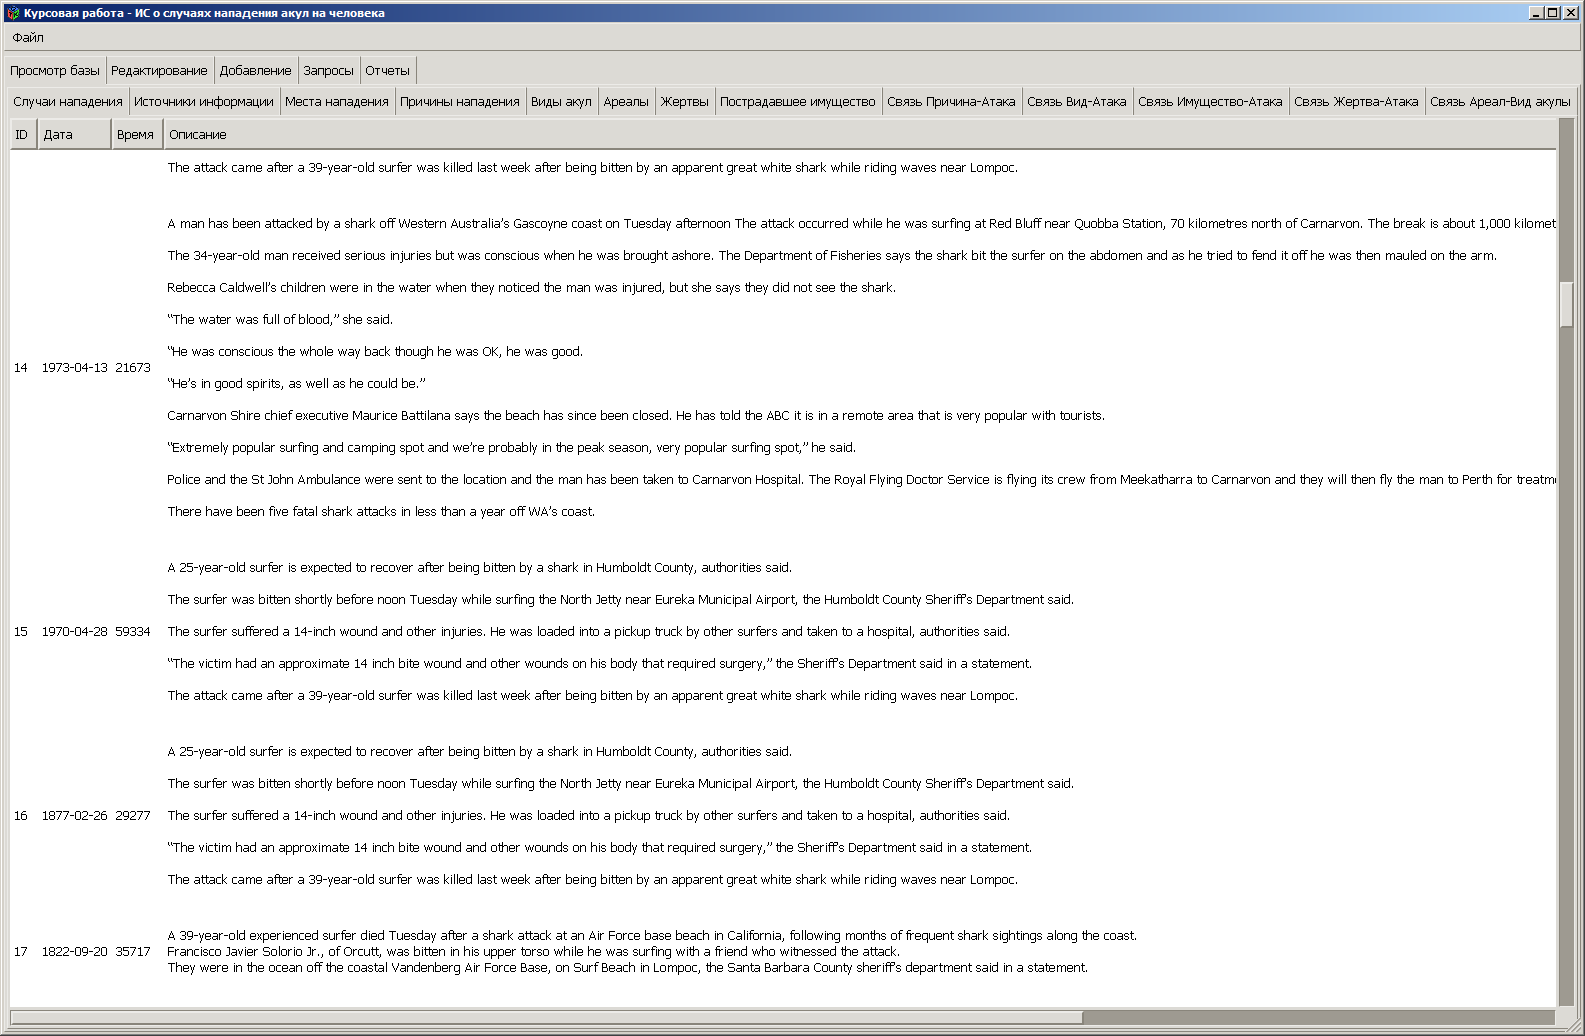
\includegraphics[width=\textwidth]{form1}
\caption{Форма <<Просмотр базы>>, таблица <<Случаи нападения>>}
\end{figure}

\begin{figure}[hb]
\centering
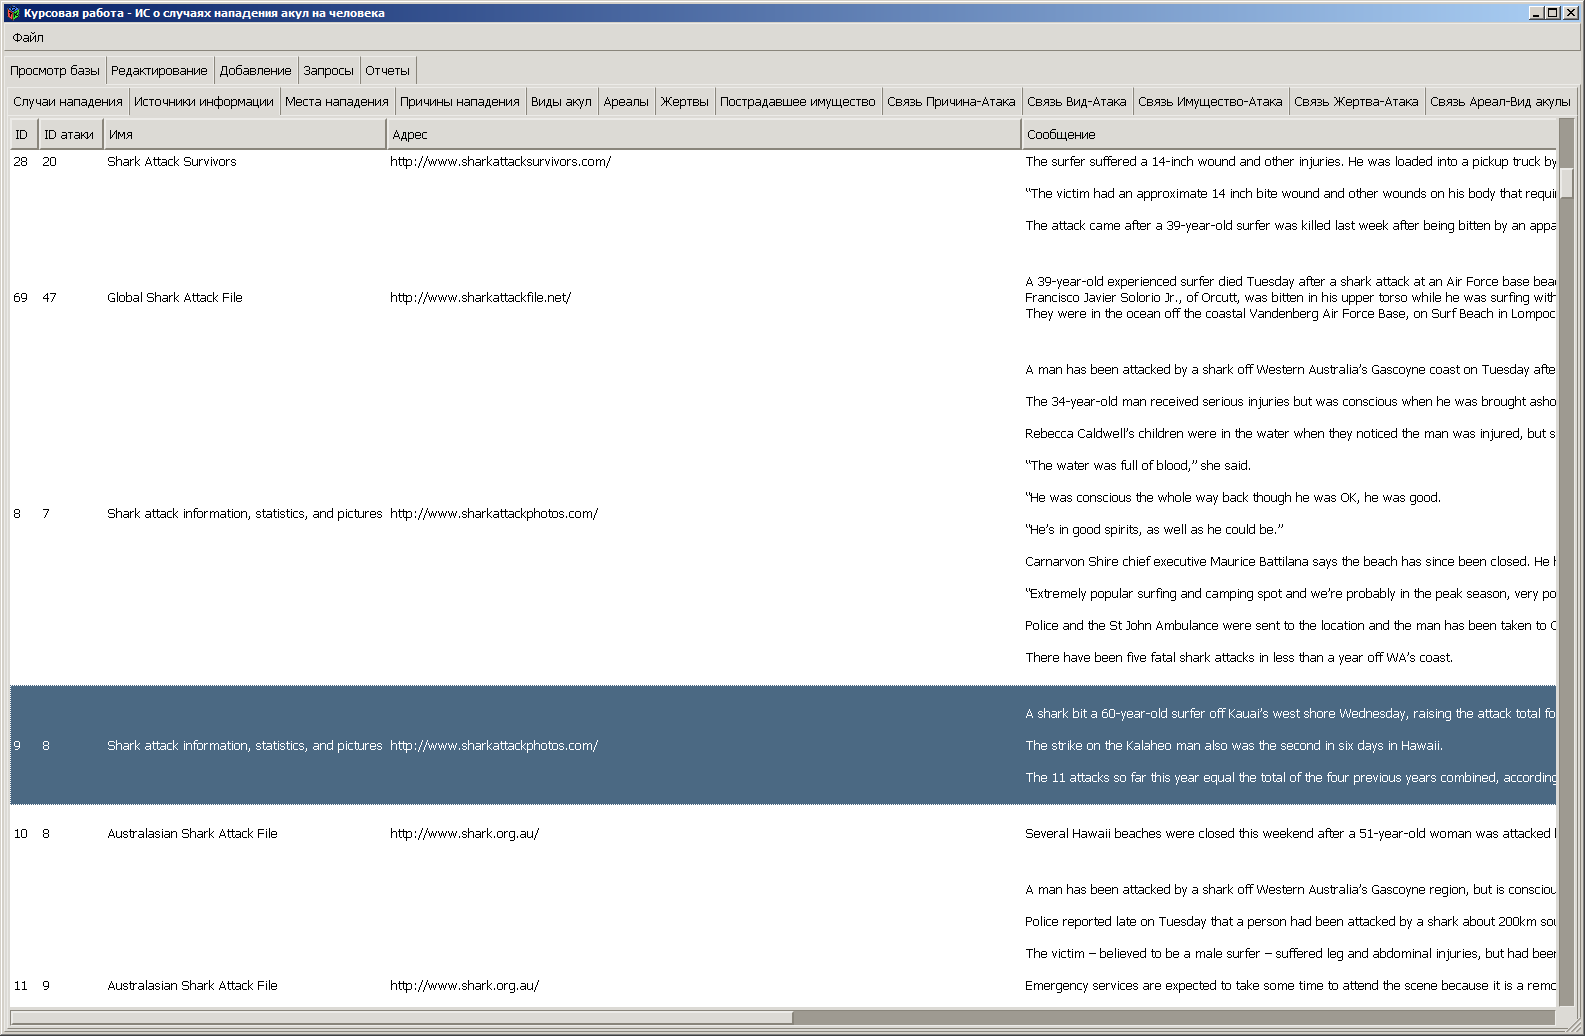
\includegraphics[width=\textwidth]{form2}
\caption{Форма <<Просмотр базы>>, таблица <<Источники информации>>}
\end{figure}

\begin{figure}[ht]
\centering
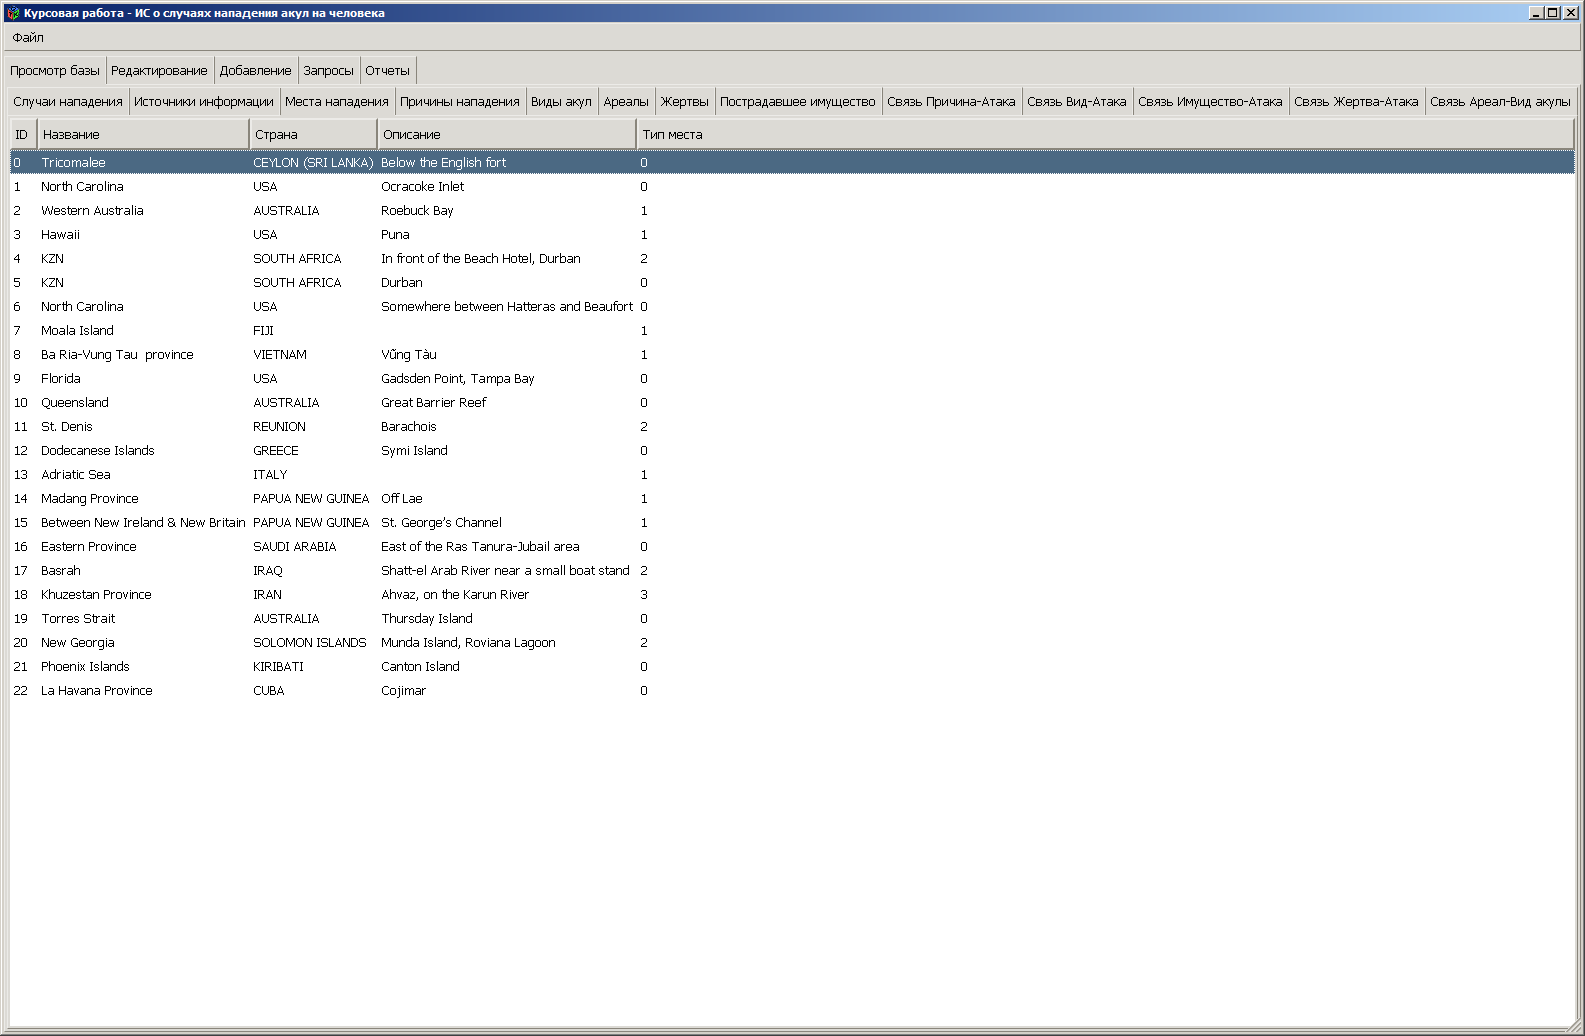
\includegraphics[width=\textwidth]{form3}
\caption{Форма <<Просмотр базы>>, таблица <<Места нападения>>}
\end{figure}

\begin{figure}[hb]
\centering
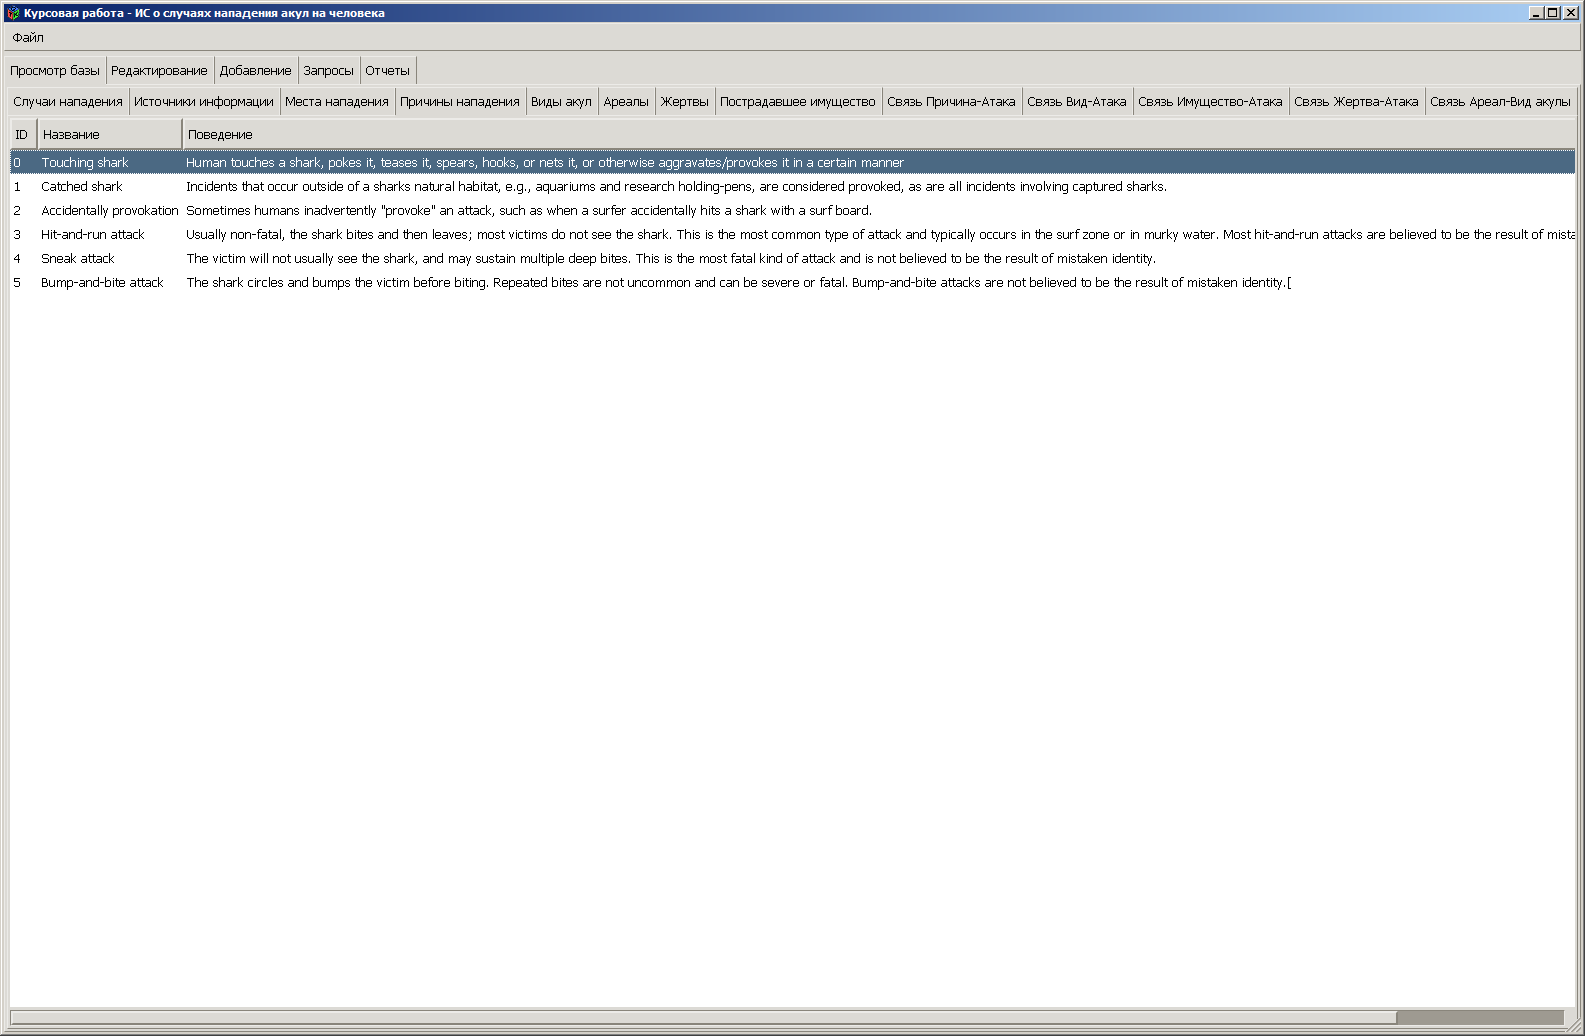
\includegraphics[width=\textwidth]{form4}
\caption{Форма <<Просмотр базы>>, таблица <<Причины нападения>>}
\end{figure}

\begin{figure}[ht]
\centering
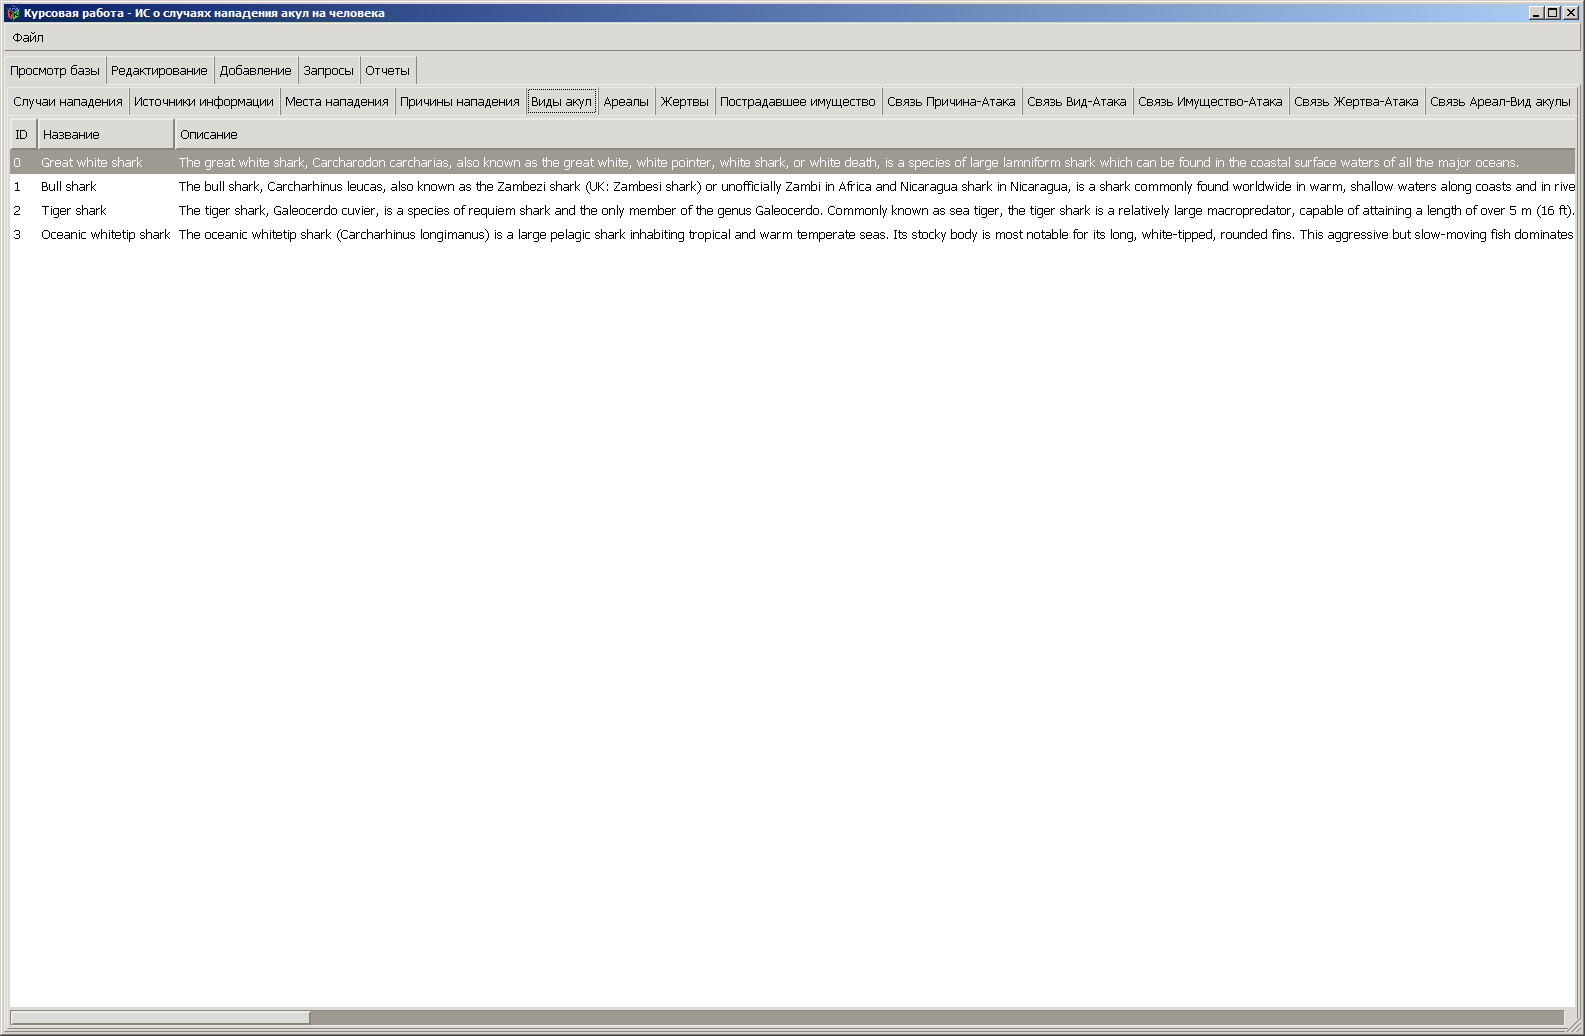
\includegraphics[width=\textwidth]{form5}
\caption{Форма <<Просмотр базы>>, таблица <<Виды акул>>}
\end{figure}

\begin{figure}[hb]
\centering
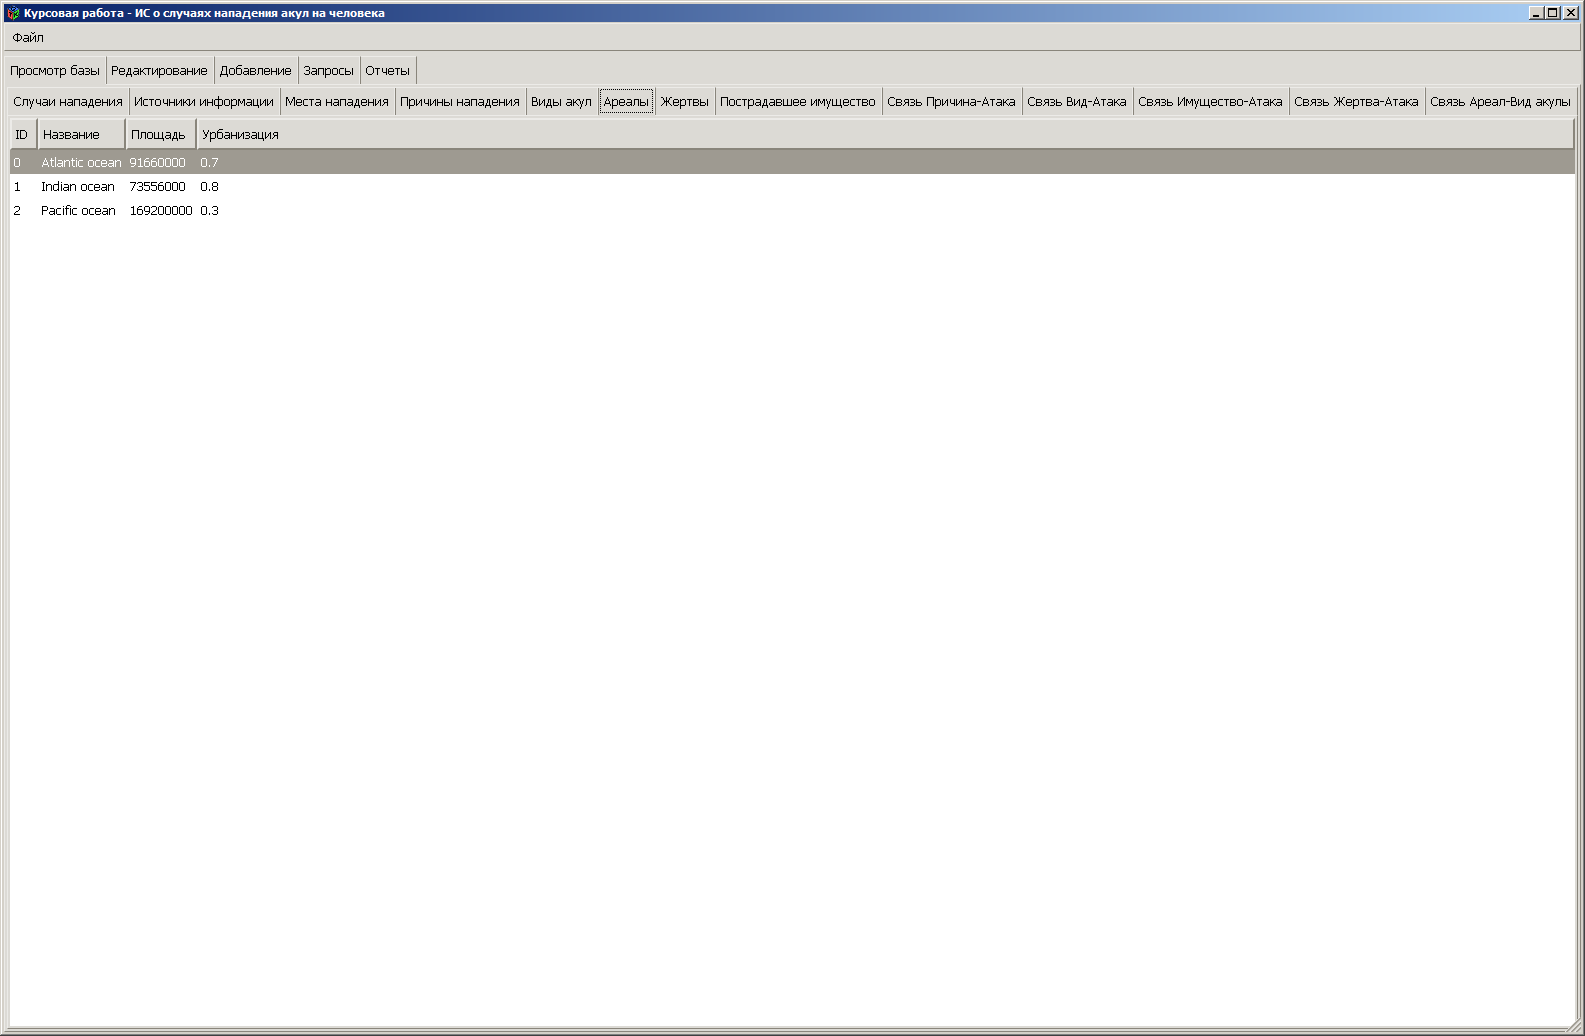
\includegraphics[width=\textwidth]{form6}
\caption{Форма <<Просмотр базы>>, таблица <<Ареалы>>}
\end{figure}

\begin{figure}[ht]
\centering
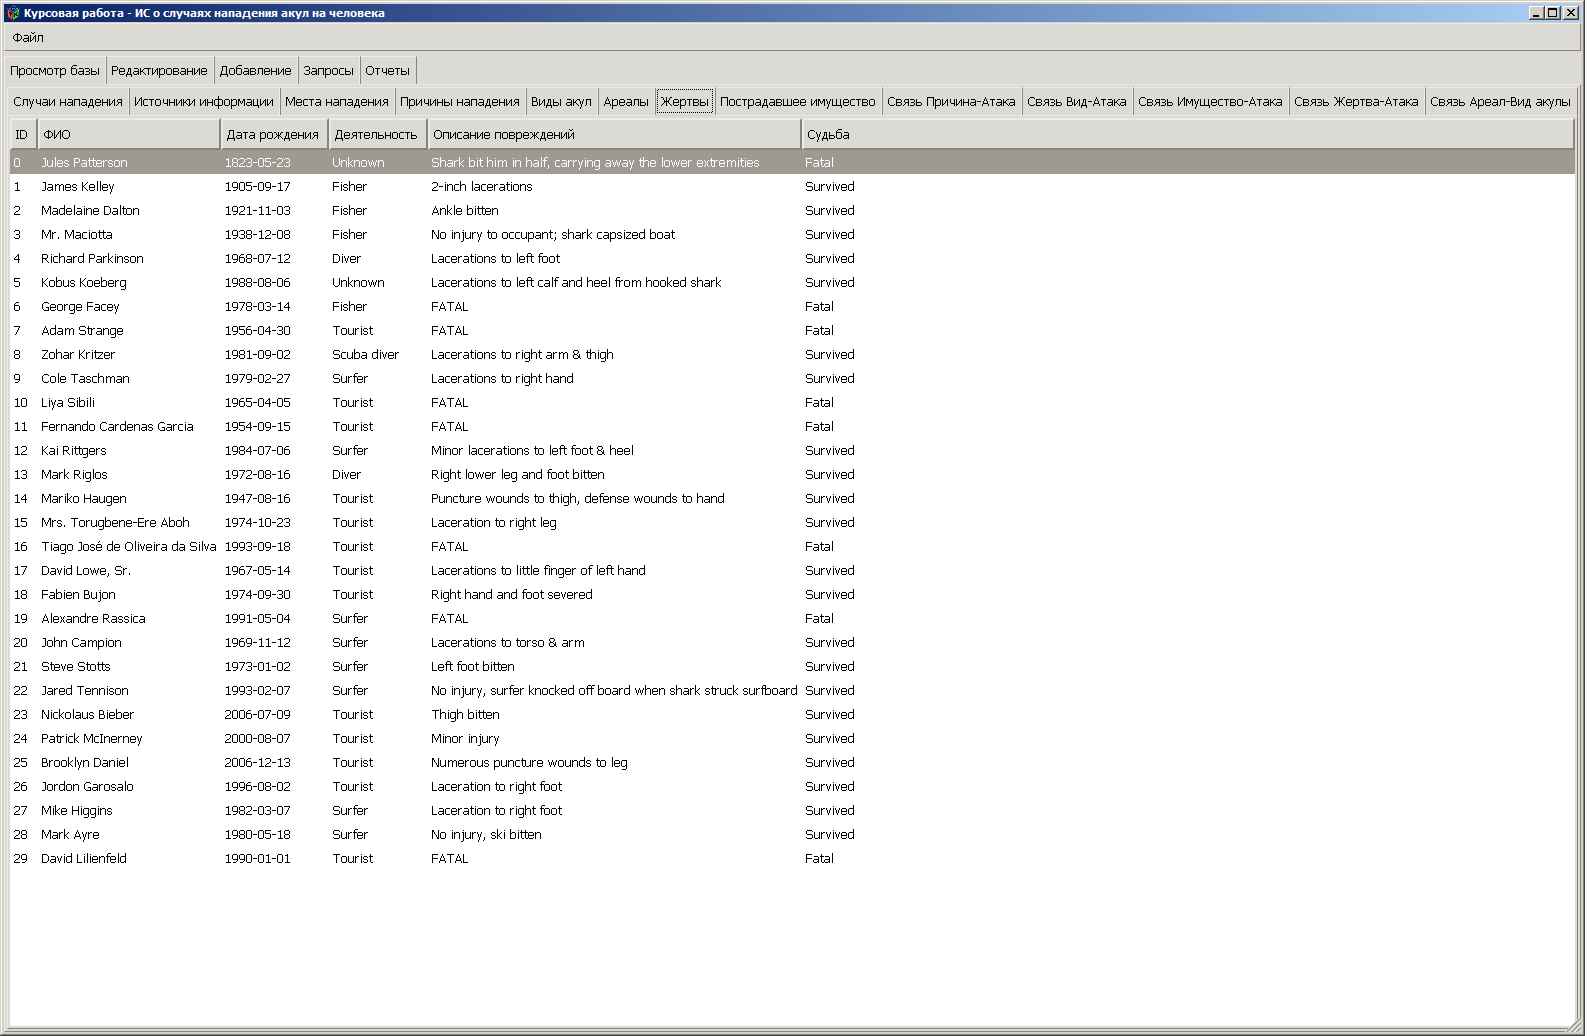
\includegraphics[width=\textwidth]{form7}
\caption{Форма <<Просмотр базы>>, таблица <<Жертвы>>}
\end{figure}


\begin{figure}[hb]
\centering
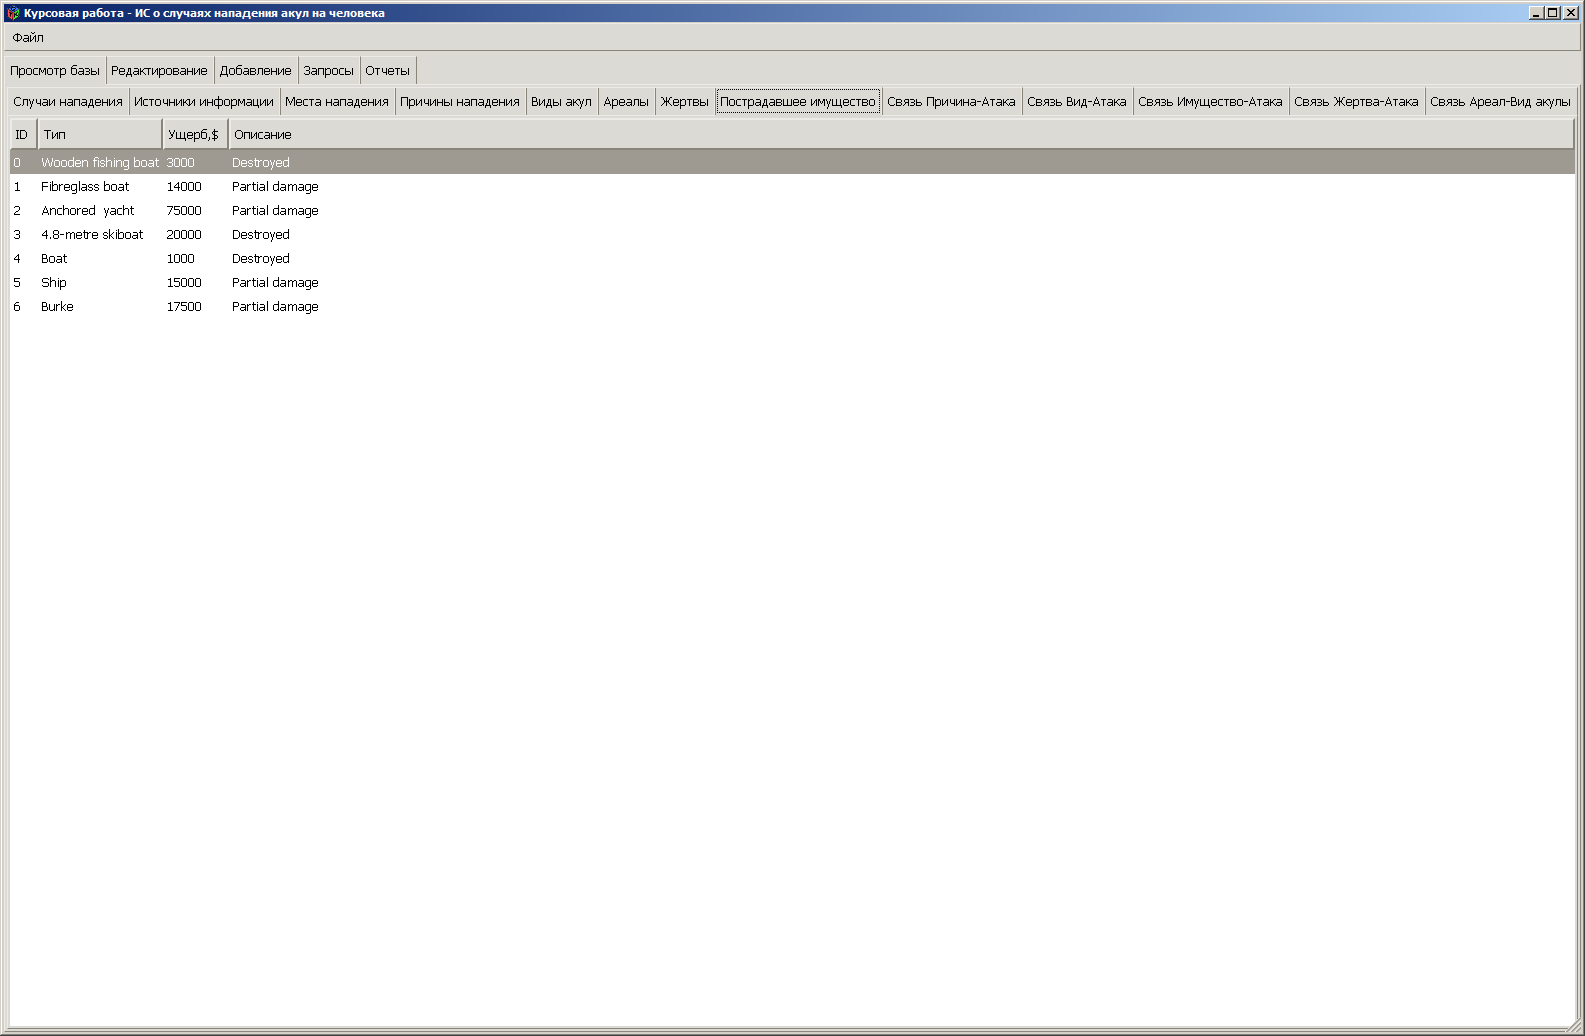
\includegraphics[width=\textwidth]{form8}
\caption{Форма <<Просмотр базы>>, таблица <<Пострадавшее имущество>>}
\end{figure}

\begin{figure}[ht]
\centering
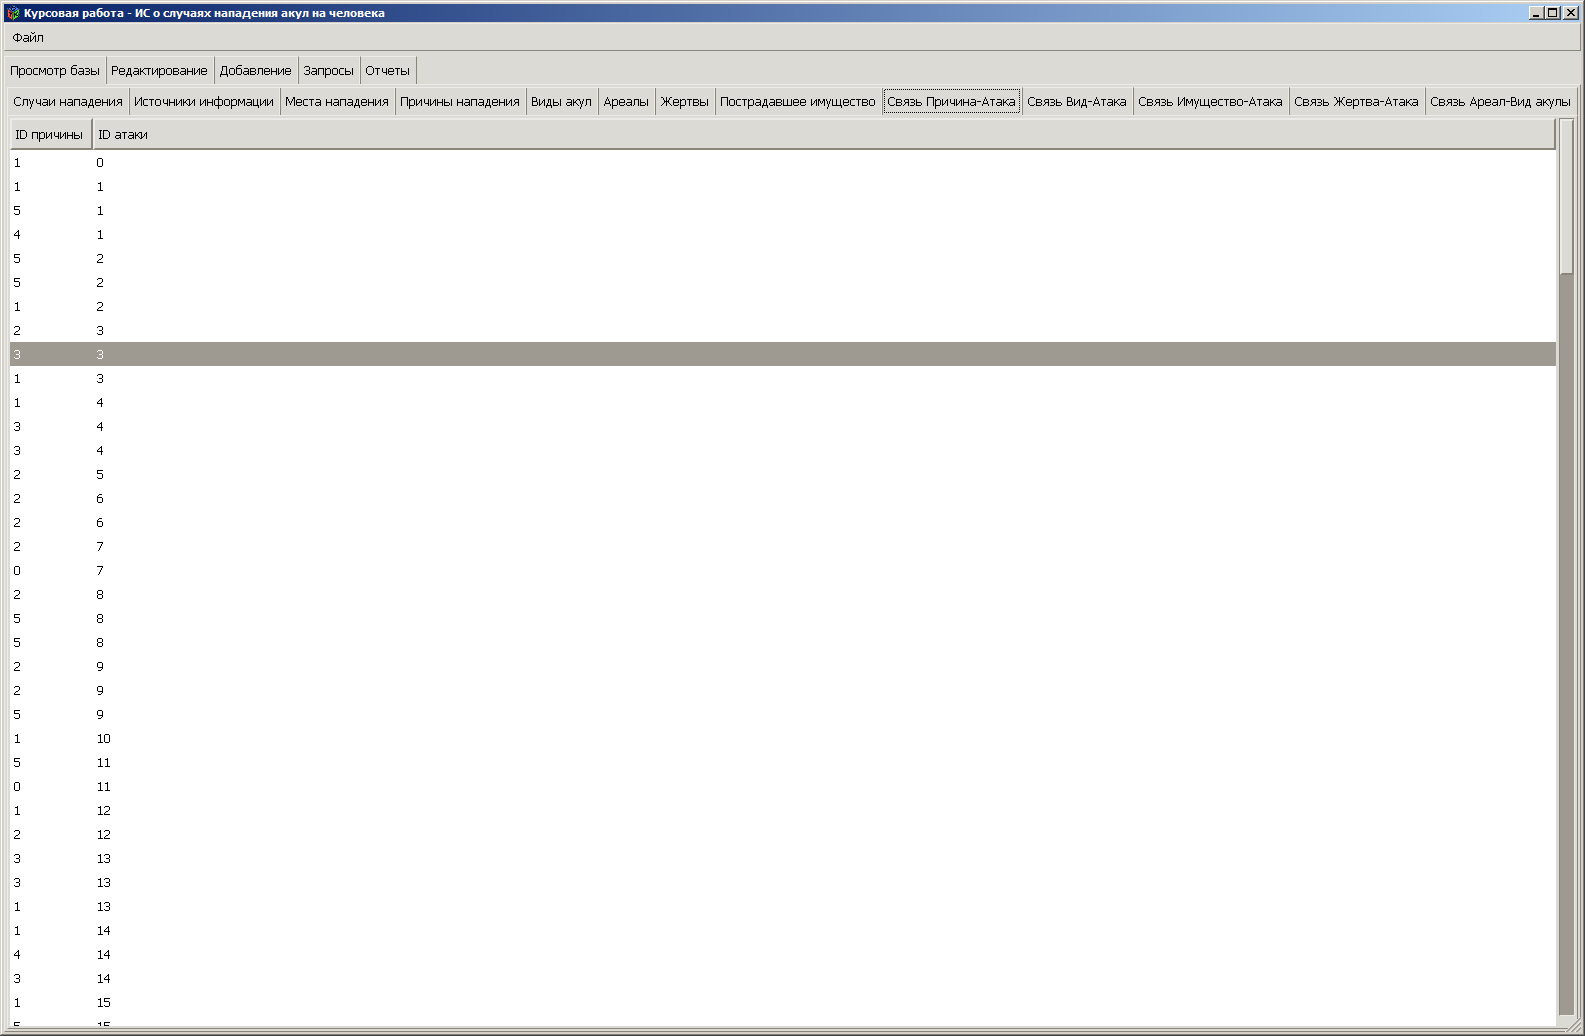
\includegraphics[width=\textwidth]{form9}
\caption{Форма <<Просмотр базы>>, таблица <<Связь Причина-Атака>>}
\end{figure}

\begin{figure}[hb]
\centering
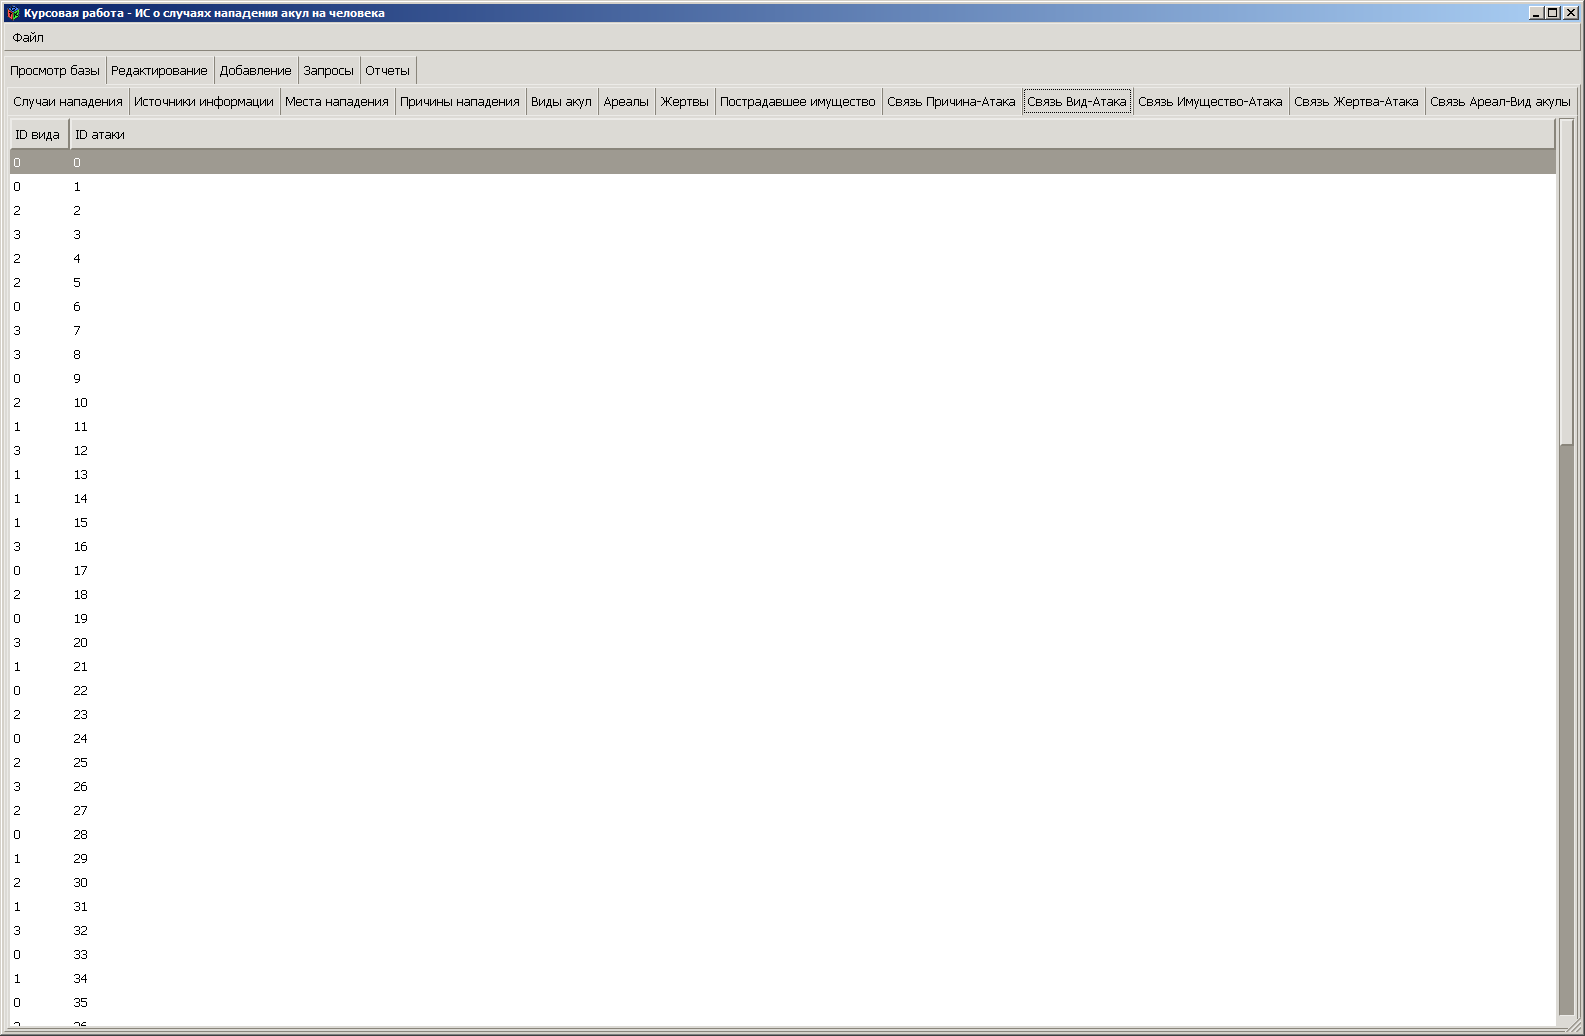
\includegraphics[width=\textwidth]{form10}
\caption{Форма <<Просмотр базы>>, таблица <<Связь Вид-Атака>>}
\end{figure}

\begin{figure}[ht]
\centering
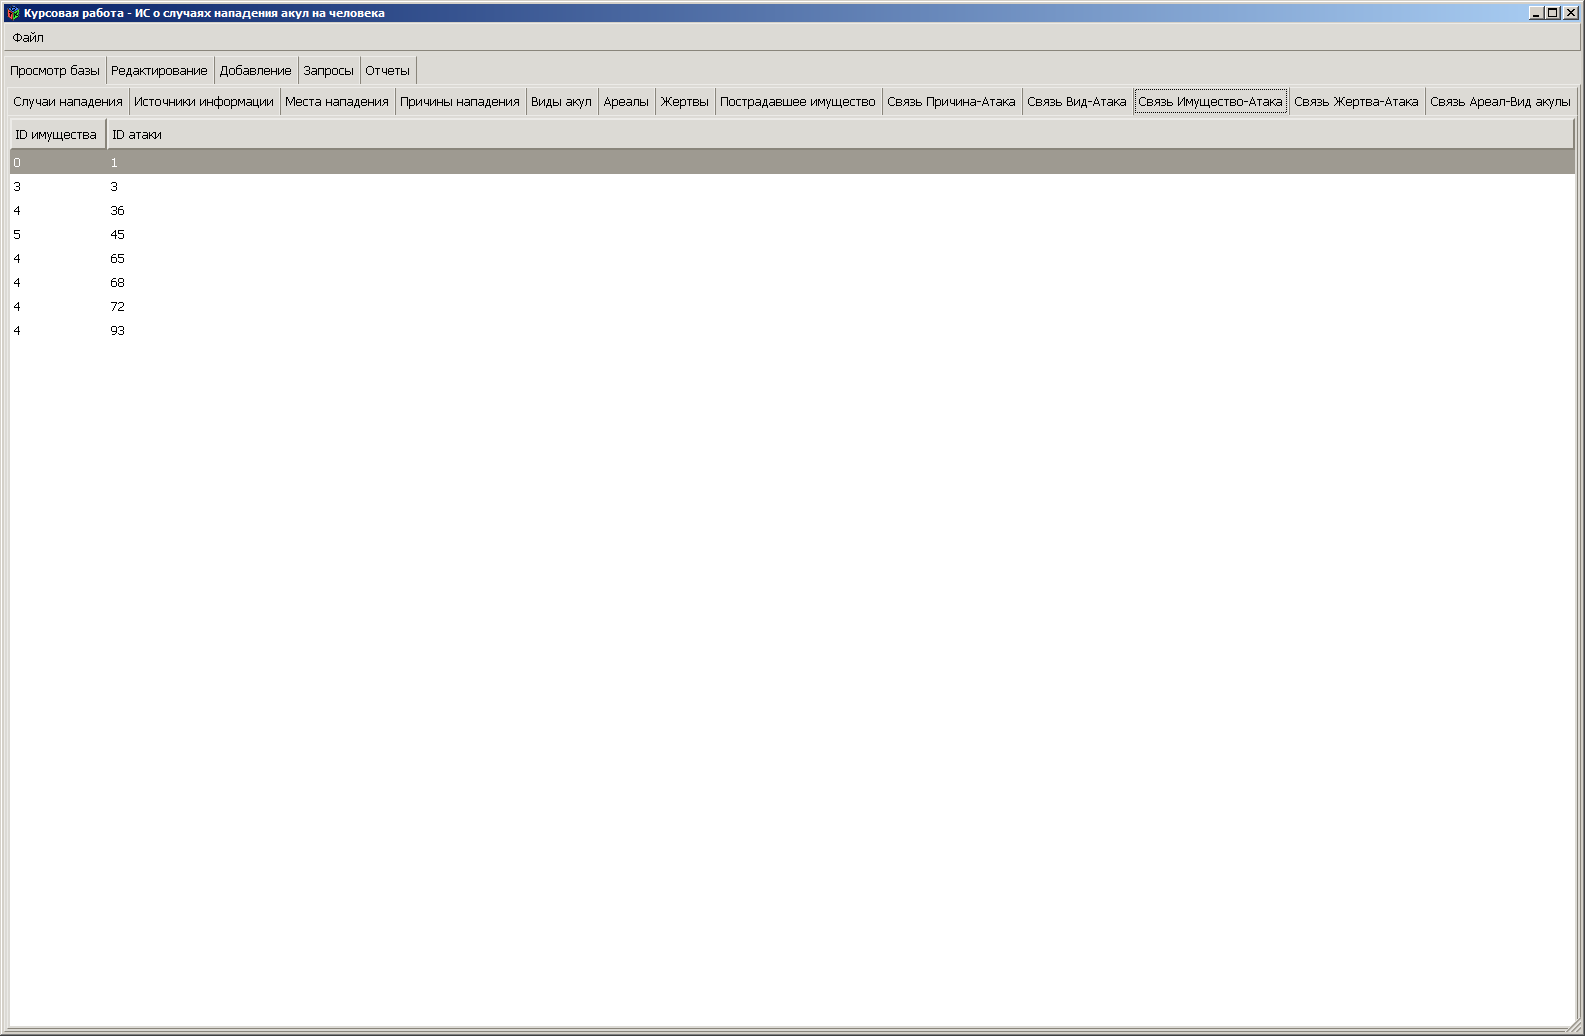
\includegraphics[width=\textwidth]{form11}
\caption{Форма <<Просмотр базы>>, таблица <<Связь Имущество-Атака>>}
\end{figure}

\begin{figure}[hb]
\centering
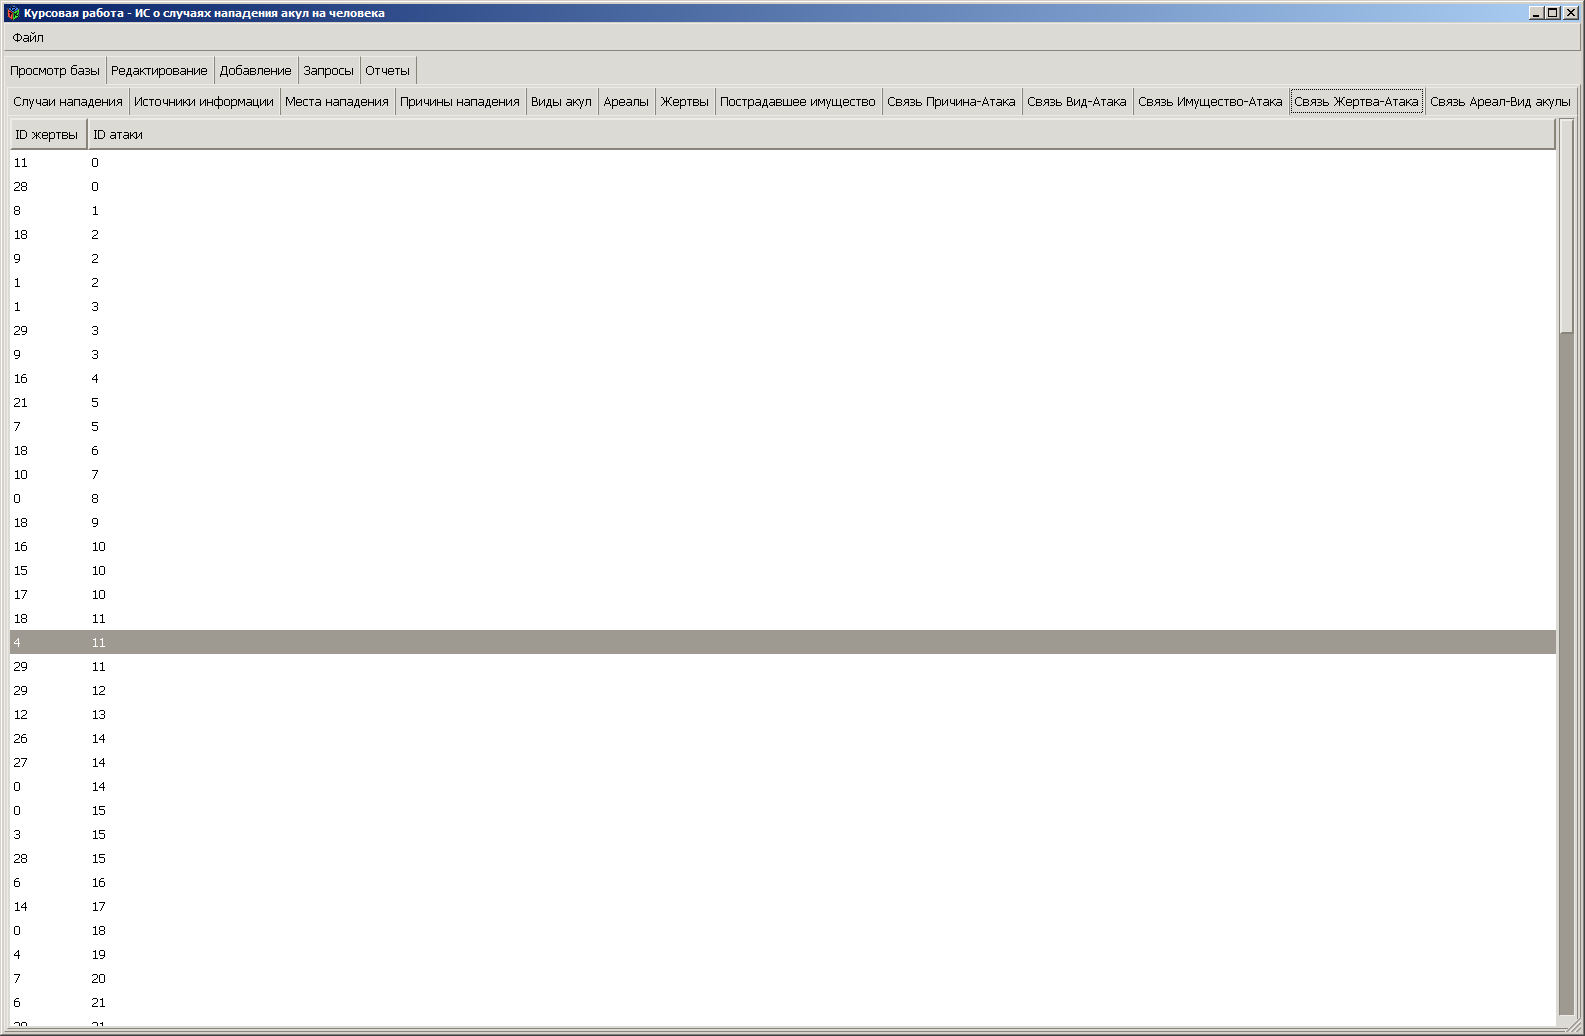
\includegraphics[width=\textwidth]{form12}
\caption{Форма <<Просмотр базы>>, таблица <<Связь Жертва-Атака>>}
\end{figure}

\begin{figure}[ht]
\centering
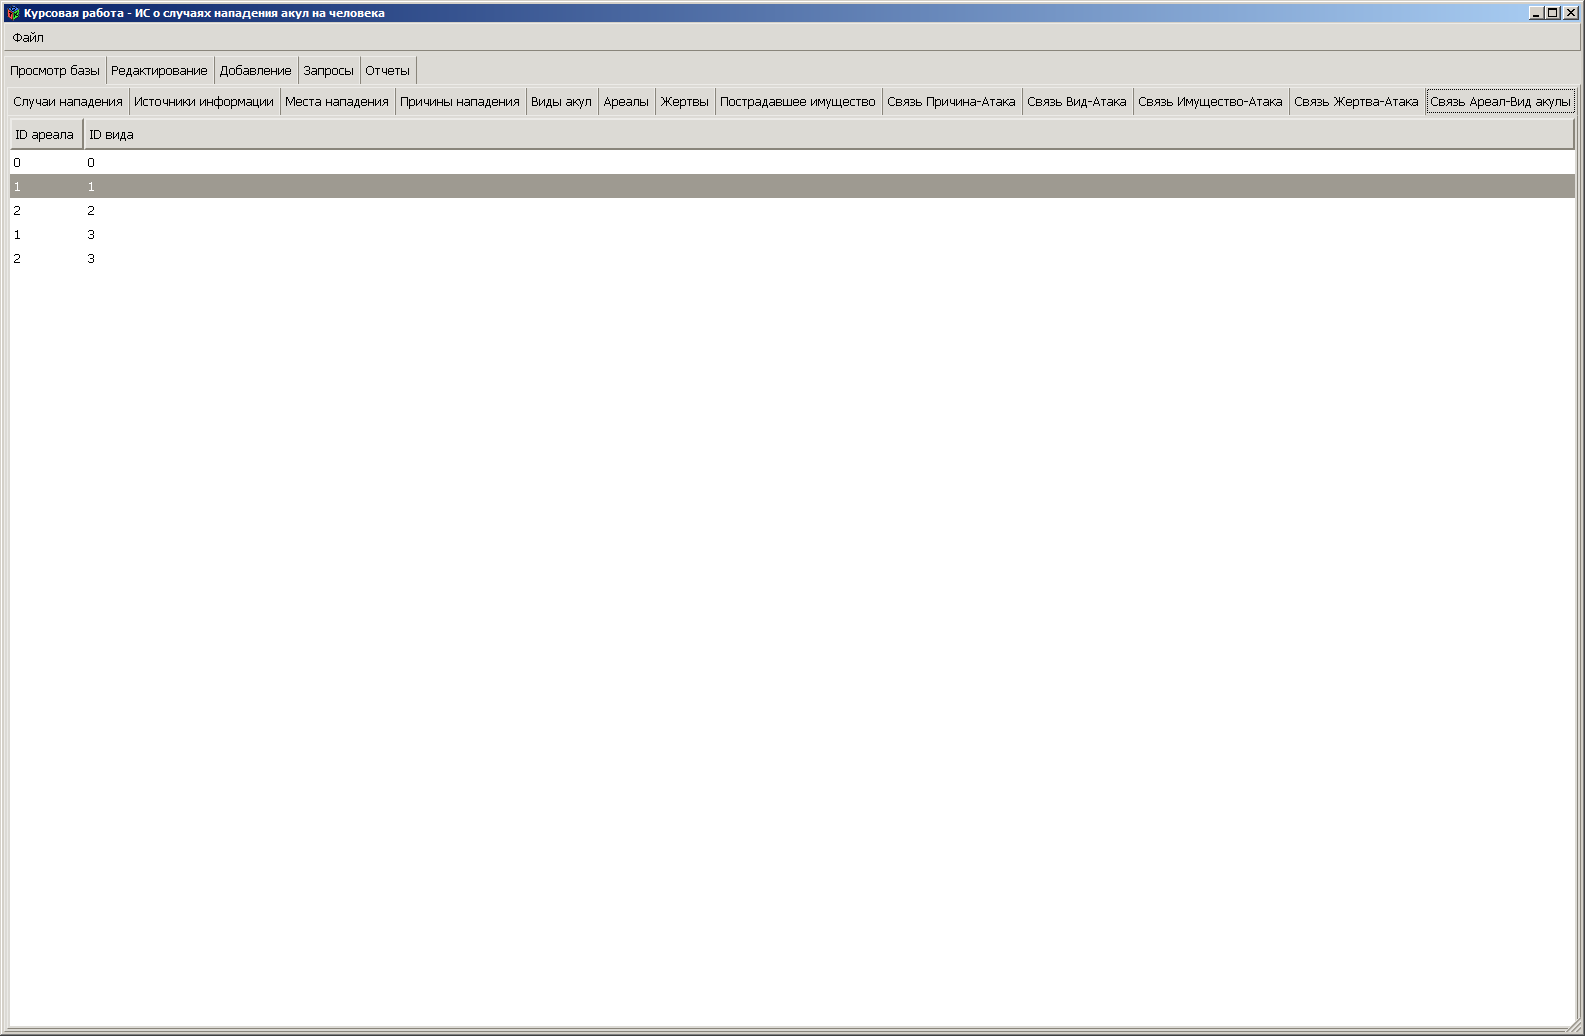
\includegraphics[width=\textwidth]{form13}
\caption{Форма <<Просмотр базы>>, таблица <<Связь Ареал-Вид акулы>>}
\end{figure}

\clearpage
\subsection{Формы редактирования таблиц}
\begin{figure}[ht]
\centering
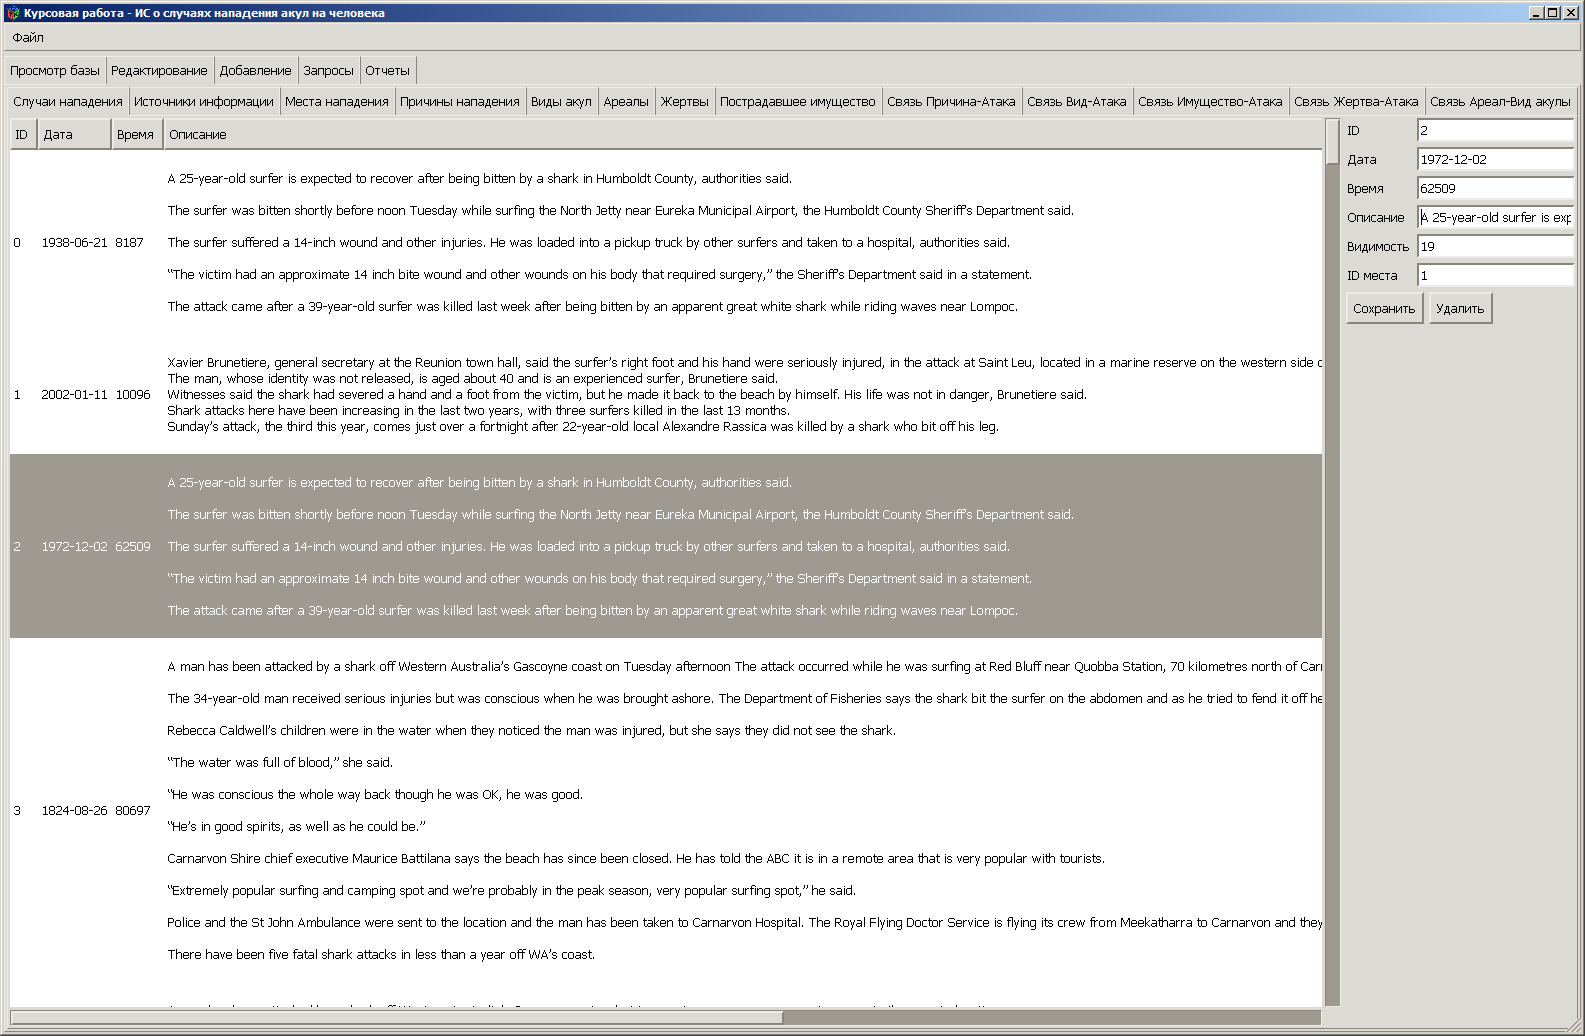
\includegraphics[width=\textwidth]{form14}
\caption{Форма <<Редактирование>>, таблица <<Случаи нападения>>}
\end{figure}

\begin{figure}[hb]
\centering
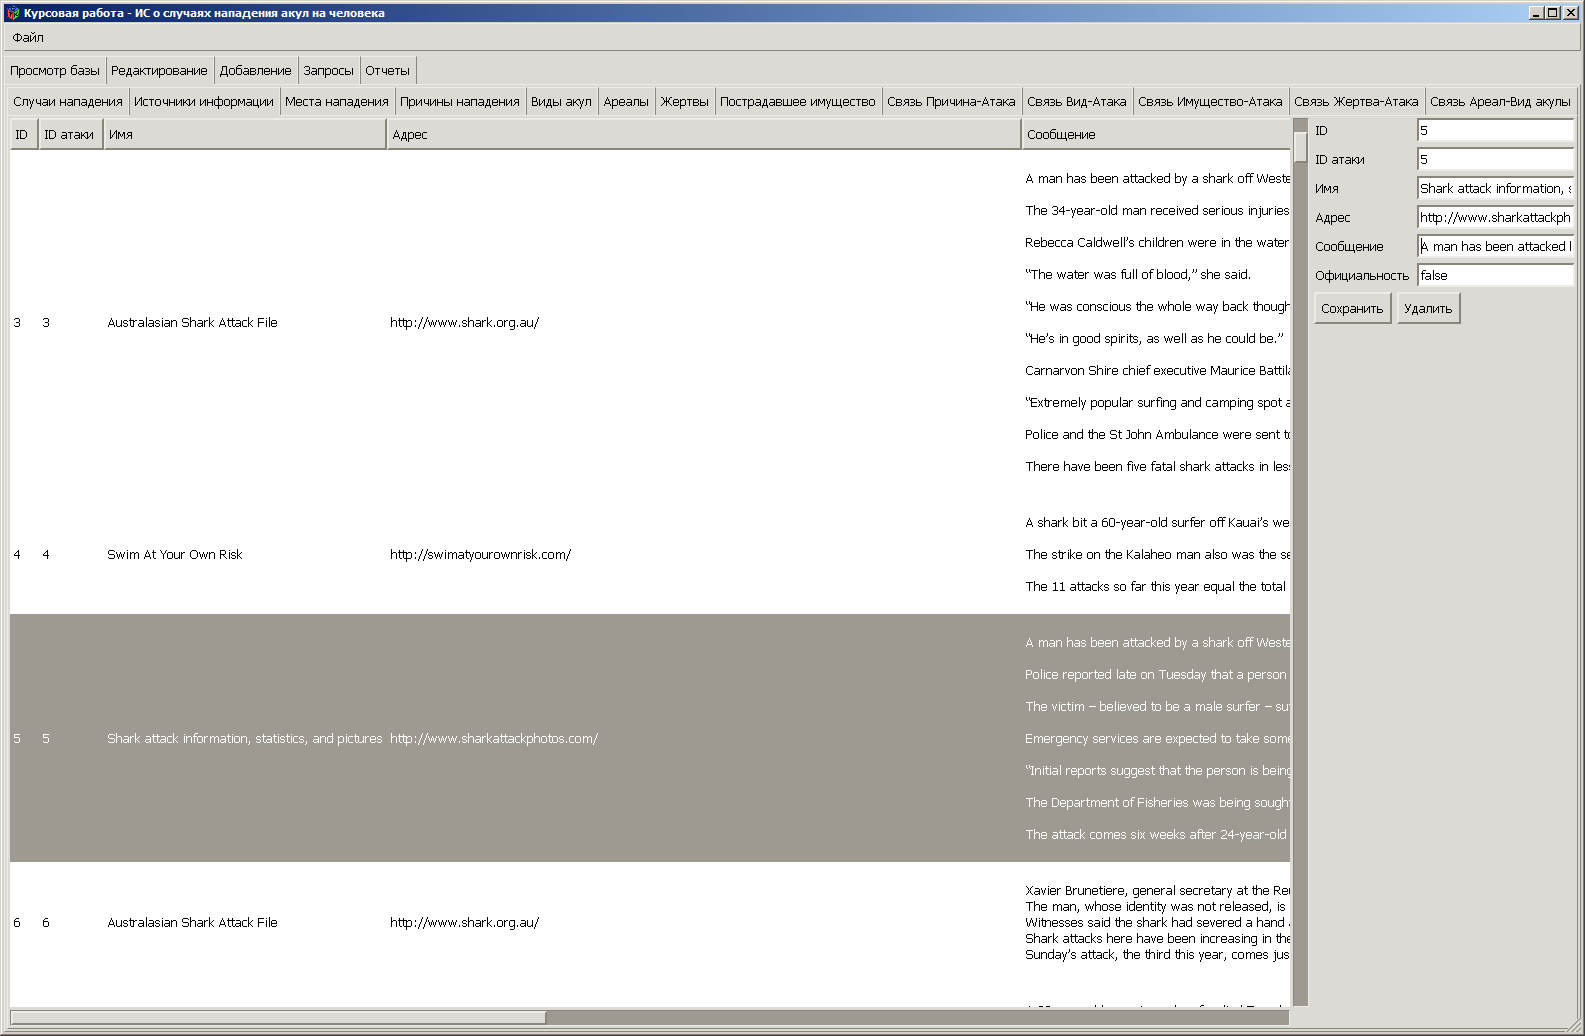
\includegraphics[width=\textwidth]{form15}
\caption{Форма <<Редактирование>>, таблица <<Источники информации>>}
\end{figure}

\begin{figure}[ht]
\centering
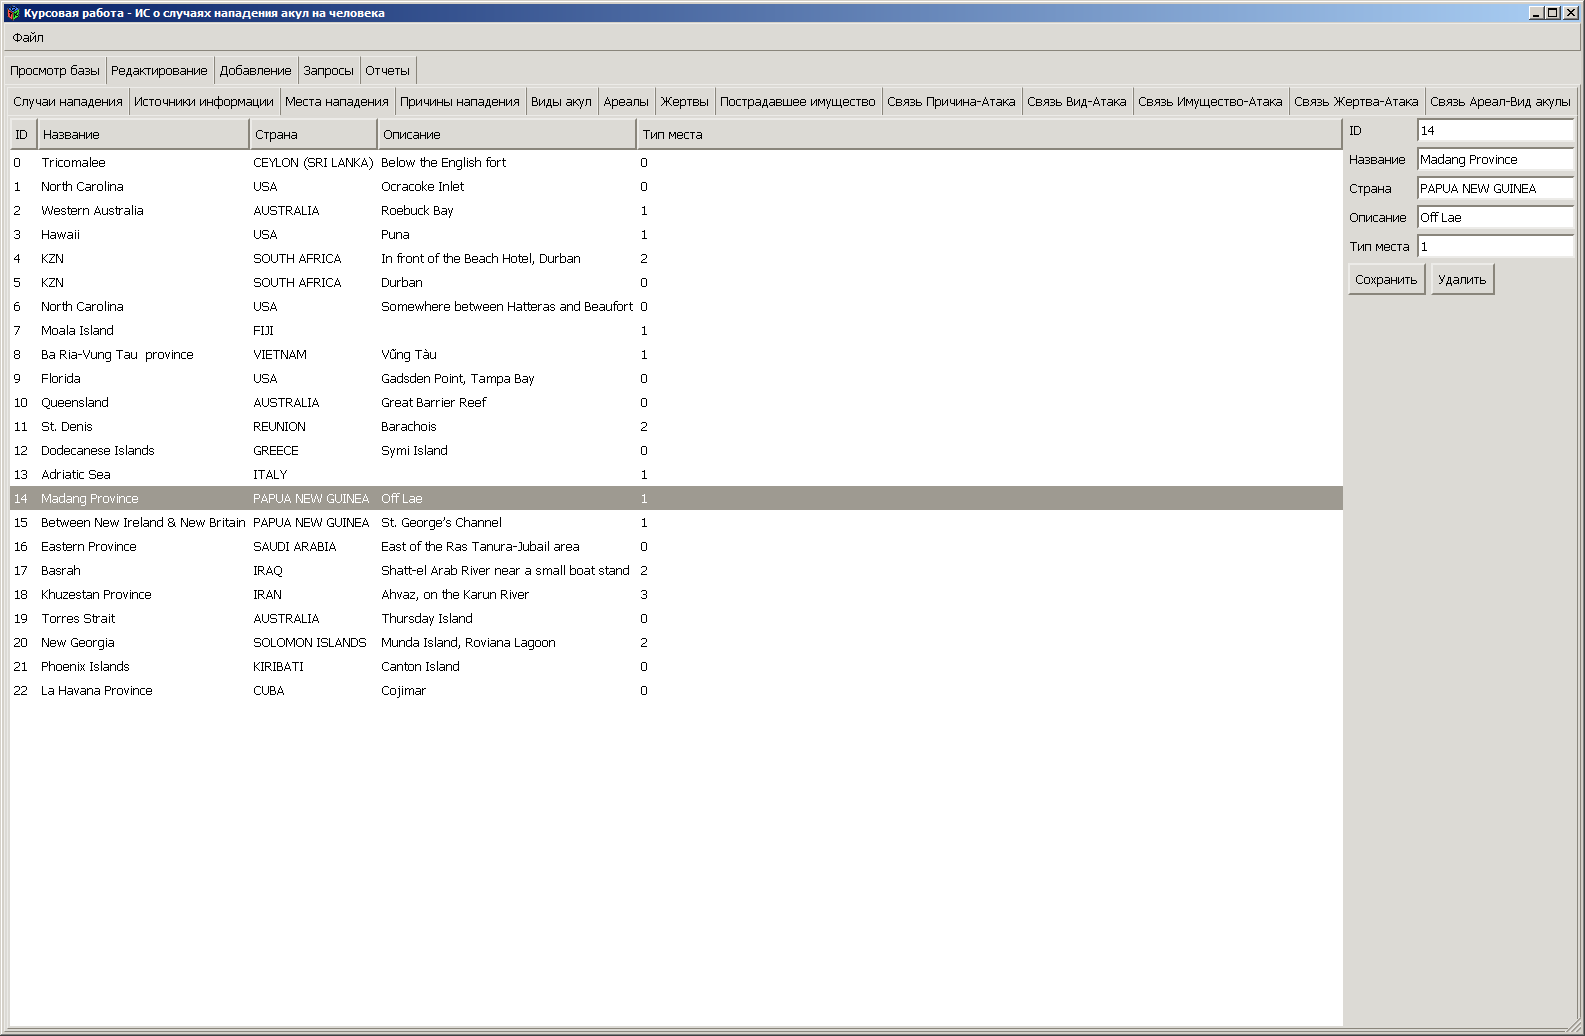
\includegraphics[width=\textwidth]{form16}
\caption{Форма <<Редактирование>>, таблица <<Места нападения>>}
\end{figure}

\begin{figure}[hb]
\centering
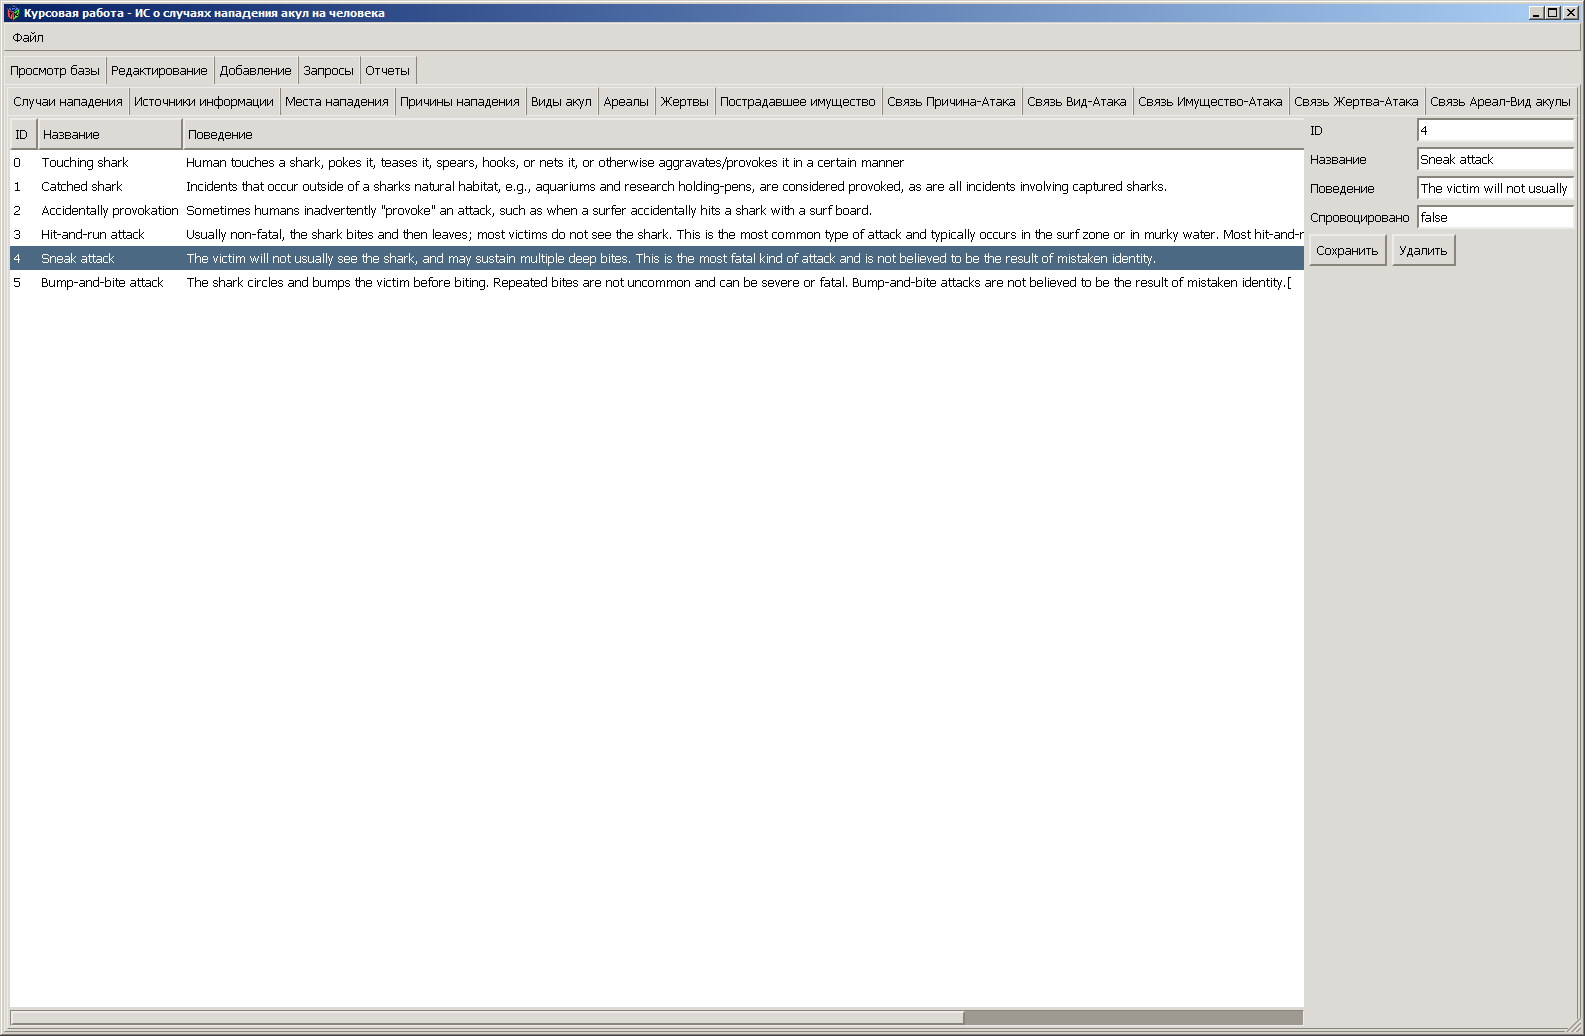
\includegraphics[width=\textwidth]{form17}
\caption{Форма <<Редактирование>>, таблица <<Причины нападения>>}
\end{figure}

\begin{figure}[ht]
\centering
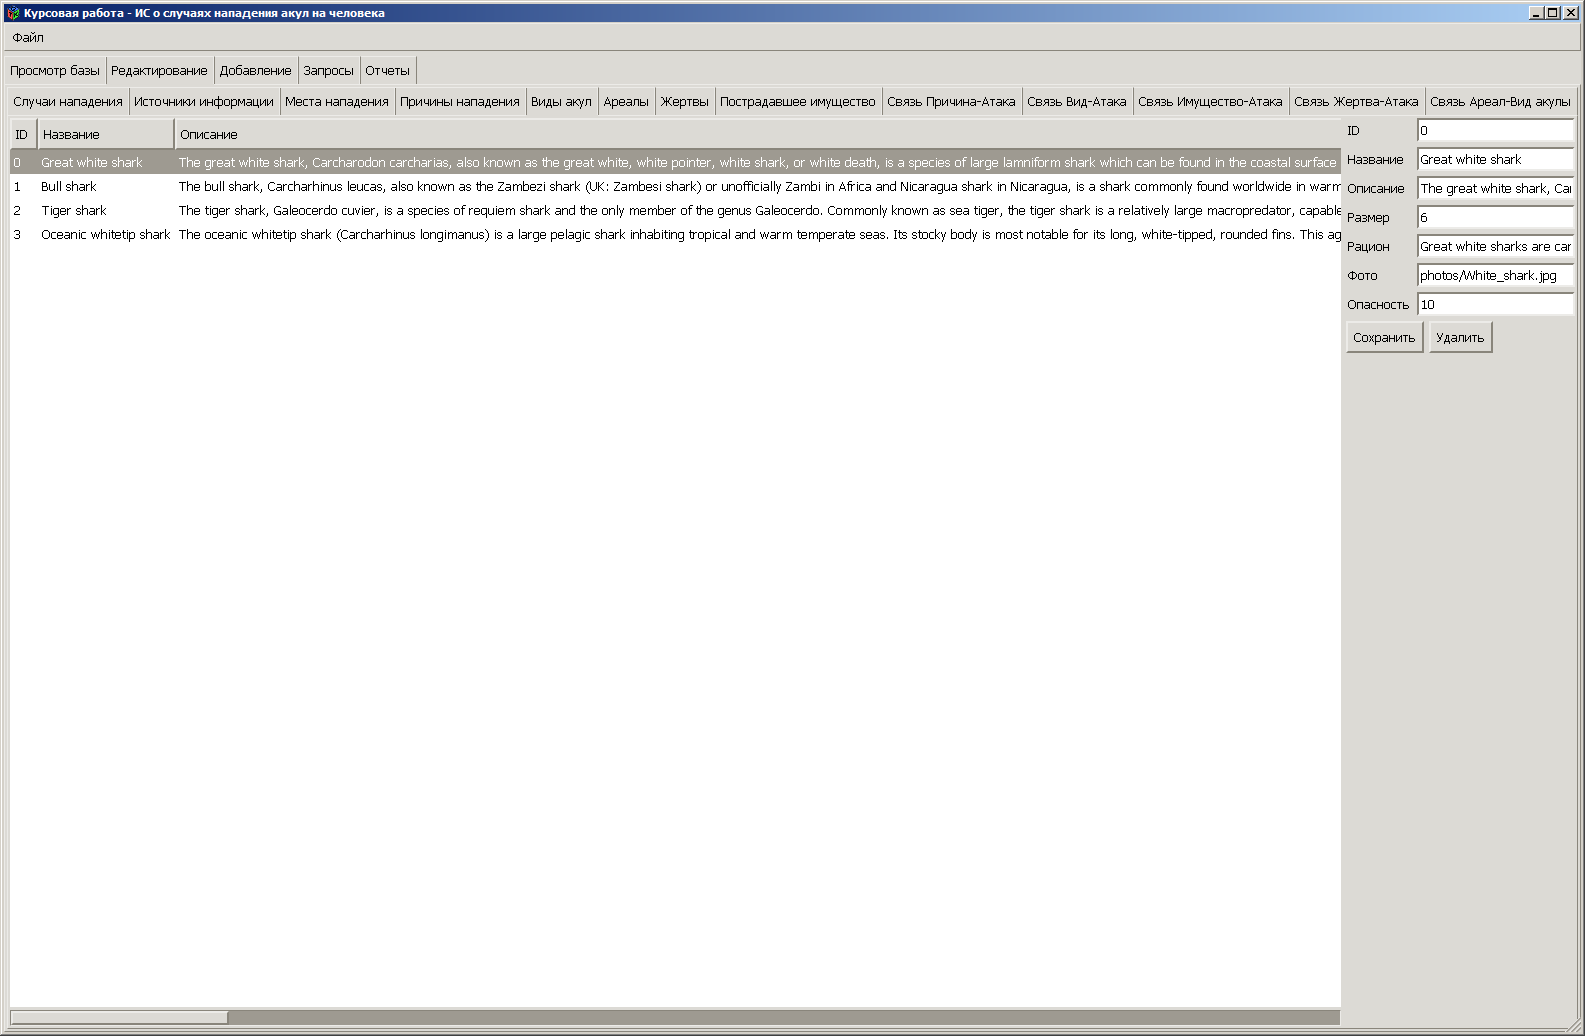
\includegraphics[width=\textwidth]{form18}
\caption{Форма <<Редактирование>>, таблица <<Виды акул>>}
\end{figure}

\begin{figure}[hb]
\centering
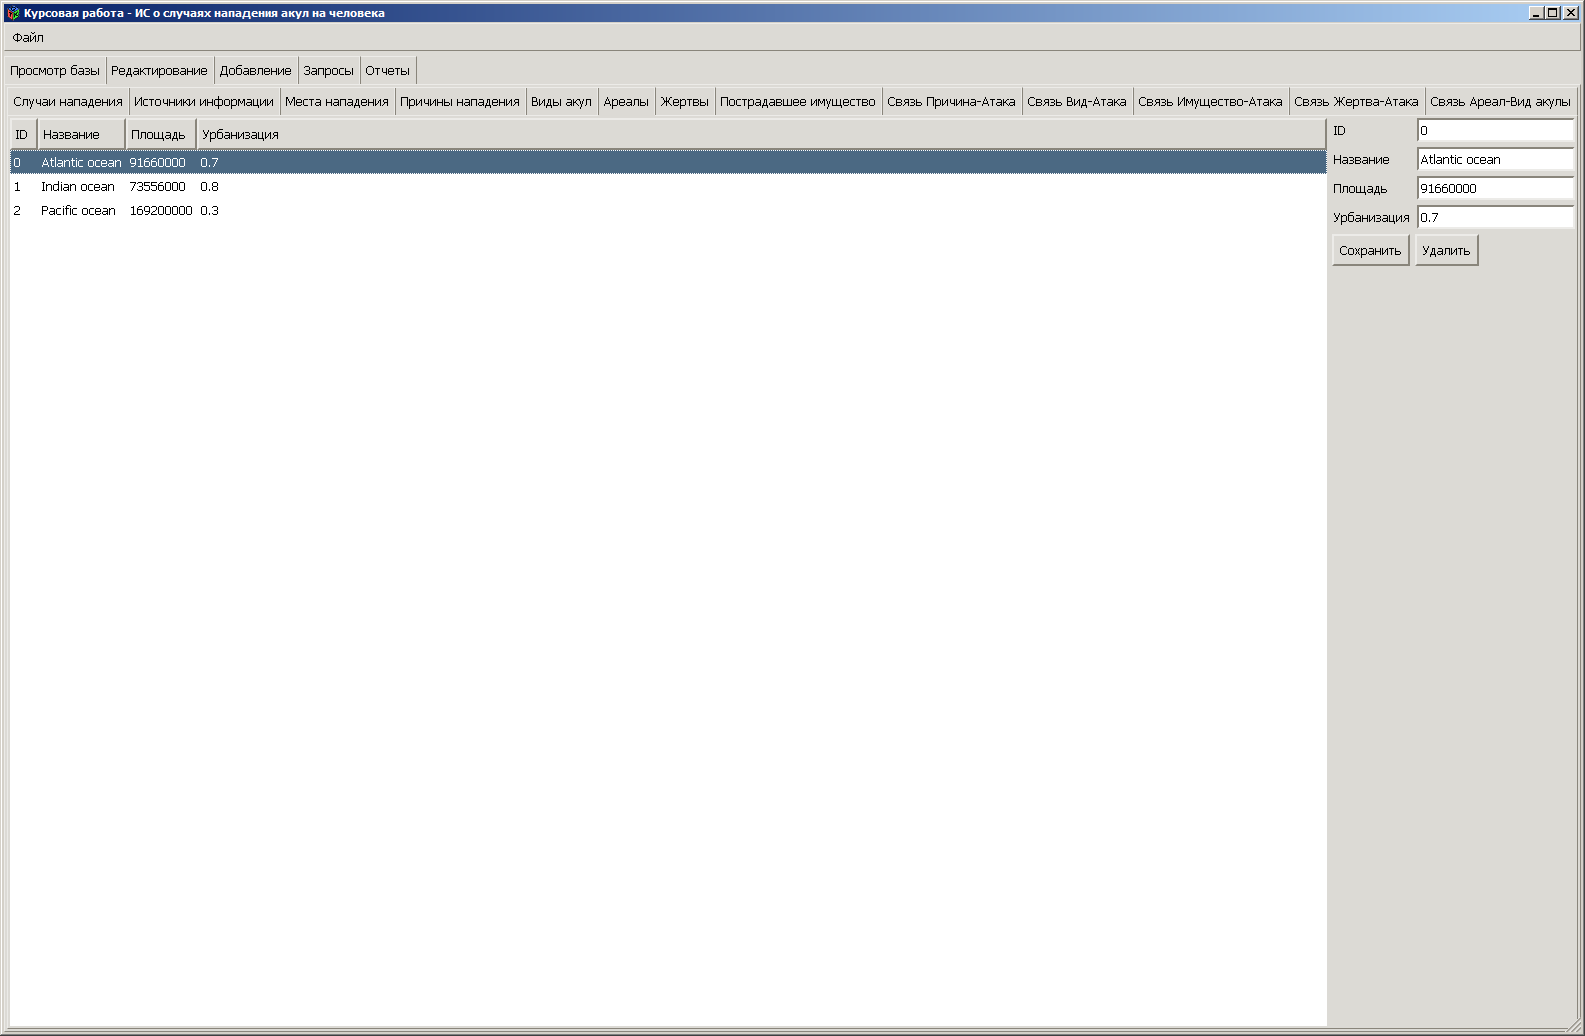
\includegraphics[width=\textwidth]{form19}
\caption{Форма <<Редактирование>>, таблица <<Ареалы>>}
\end{figure}

\begin{figure}[ht]
\centering
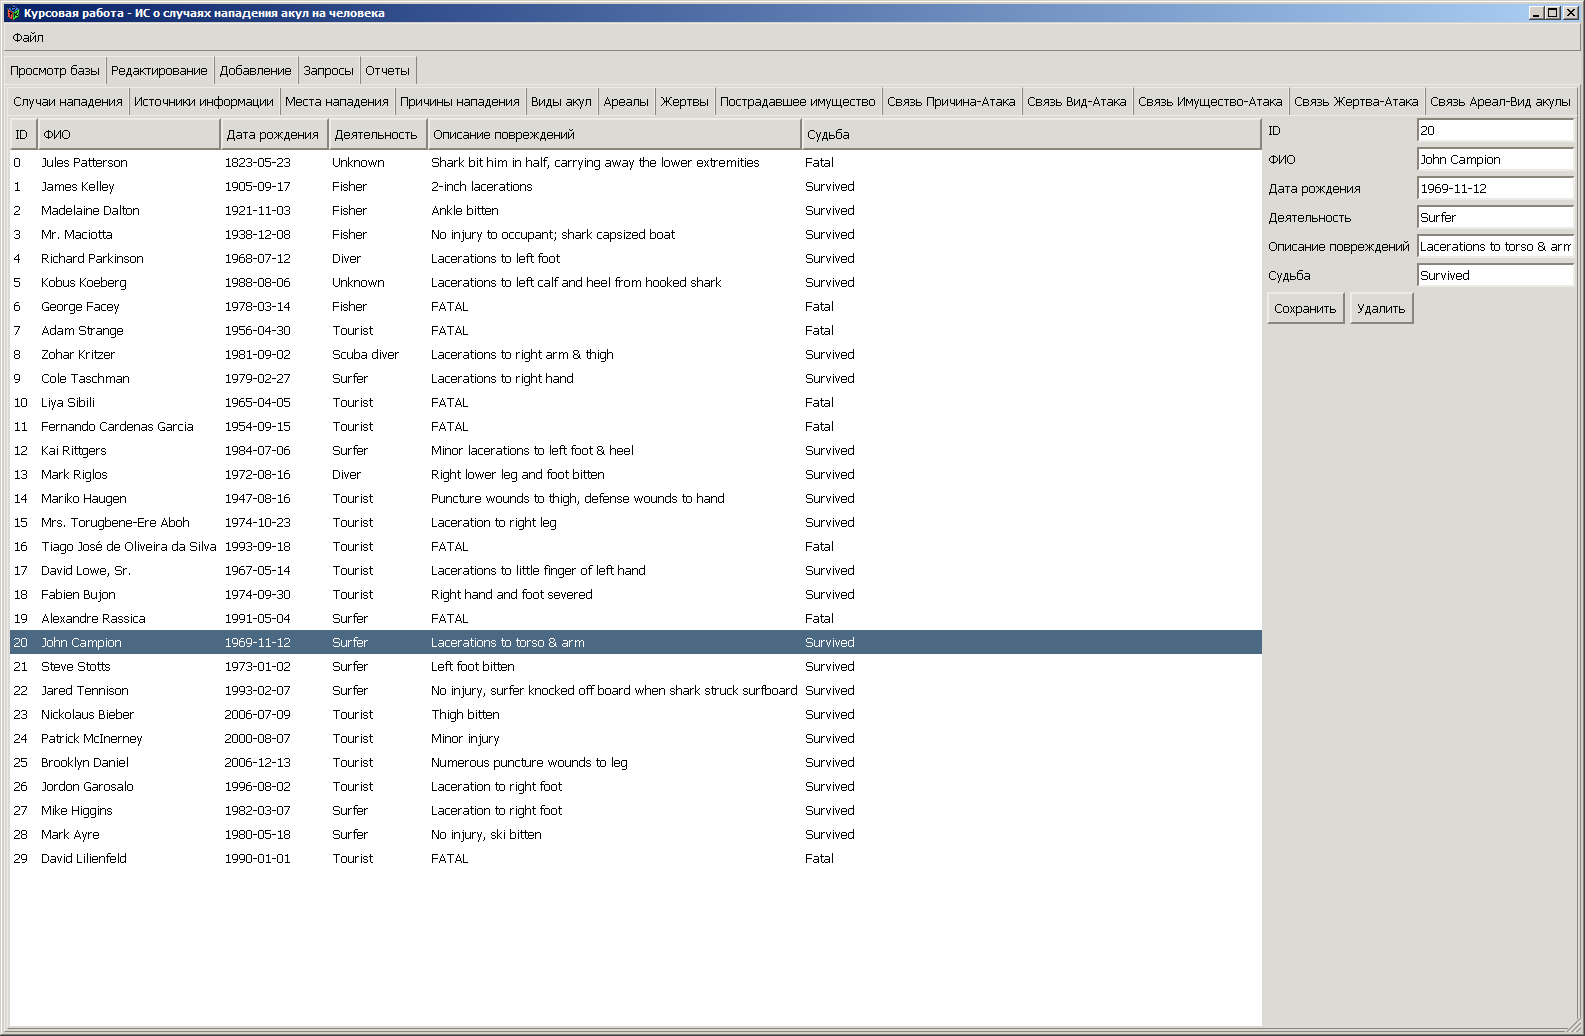
\includegraphics[width=\textwidth]{form20}
\caption{Форма <<Редактирование>>, таблица <<Жертвы>>}
\end{figure}

\begin{figure}[hb]
\centering
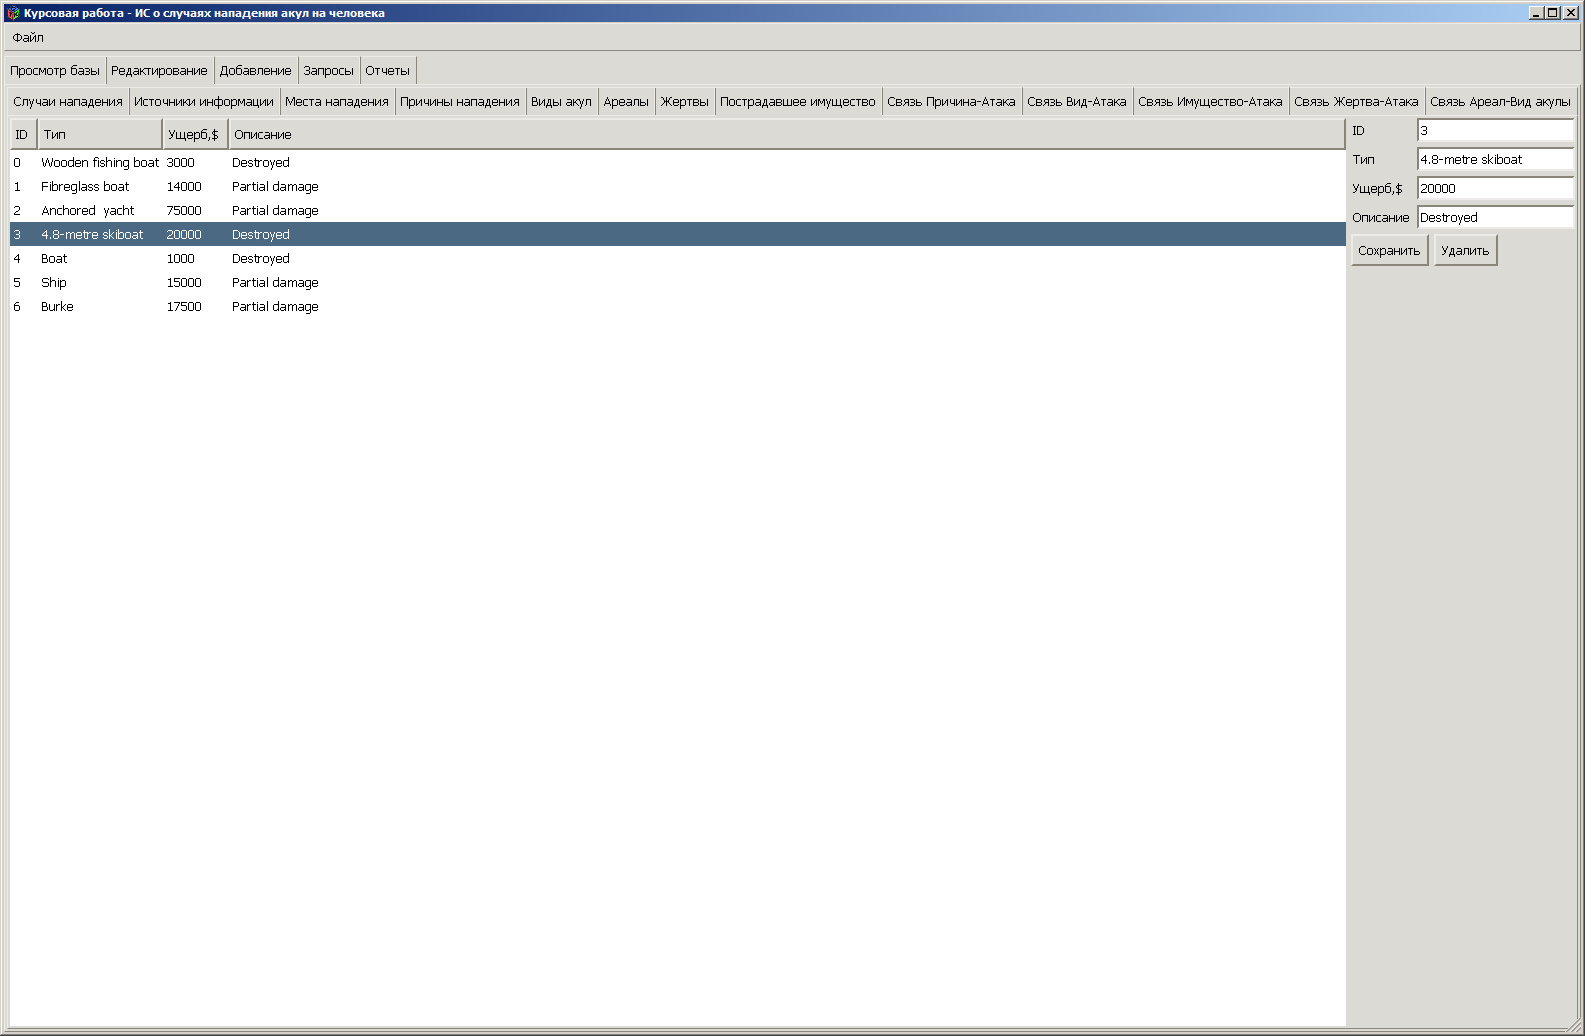
\includegraphics[width=\textwidth]{form21}
\caption{Форма <<Редактирование>>, таблица <<Пострадавшее имущество>>}
\end{figure}

\begin{figure}[ht]
\centering
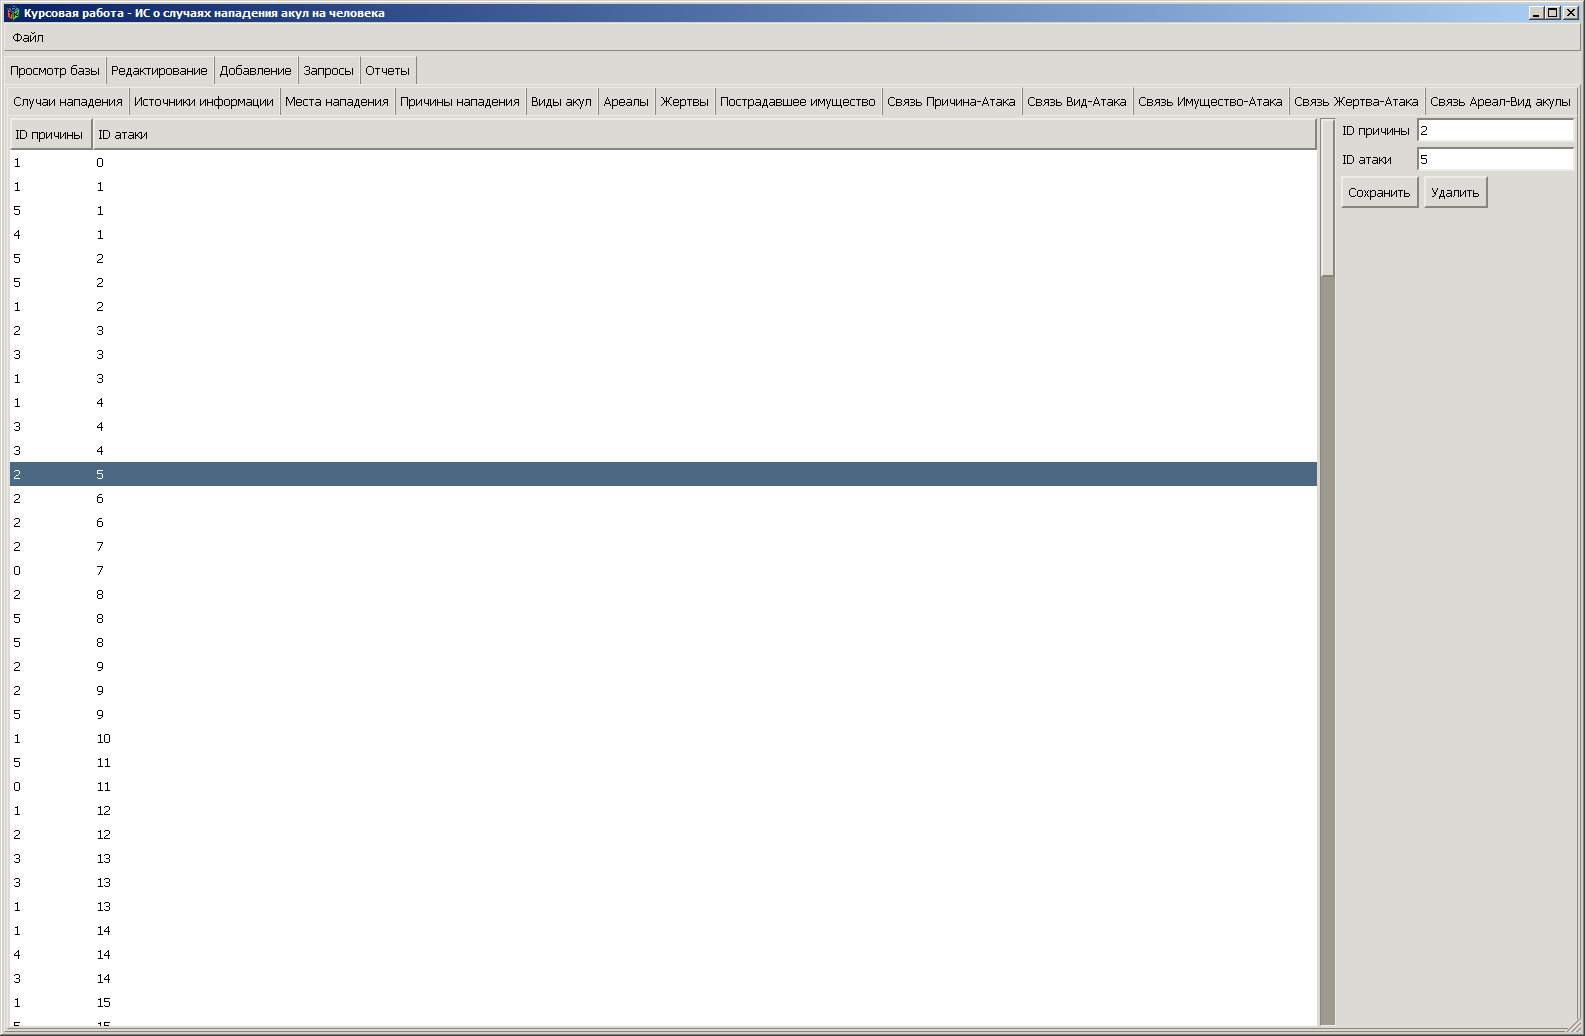
\includegraphics[width=\textwidth]{form22}
\caption{Форма <<Редактирование>>, таблица <<Связь Причина-Атака>>}
\end{figure}

\begin{figure}[hb]
\centering
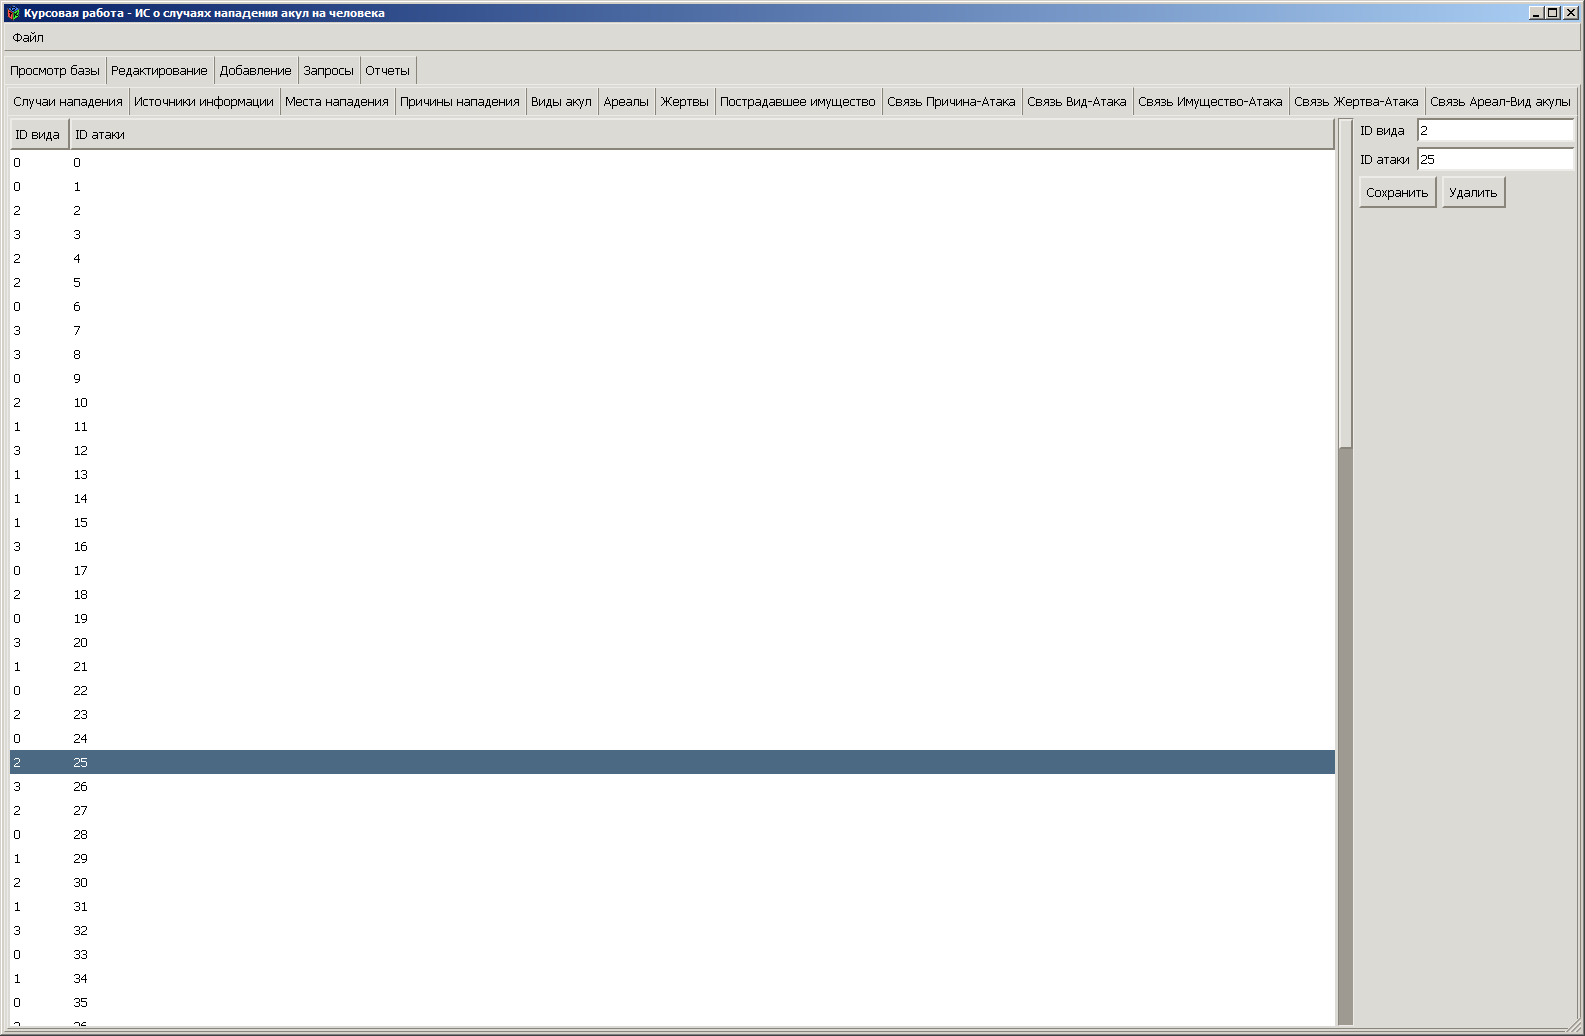
\includegraphics[width=\textwidth]{form23}
\caption{Форма <<Редактирование>>, таблица <<Связь Вид-Атака>>}
\end{figure}

\begin{figure}[ht]
\centering
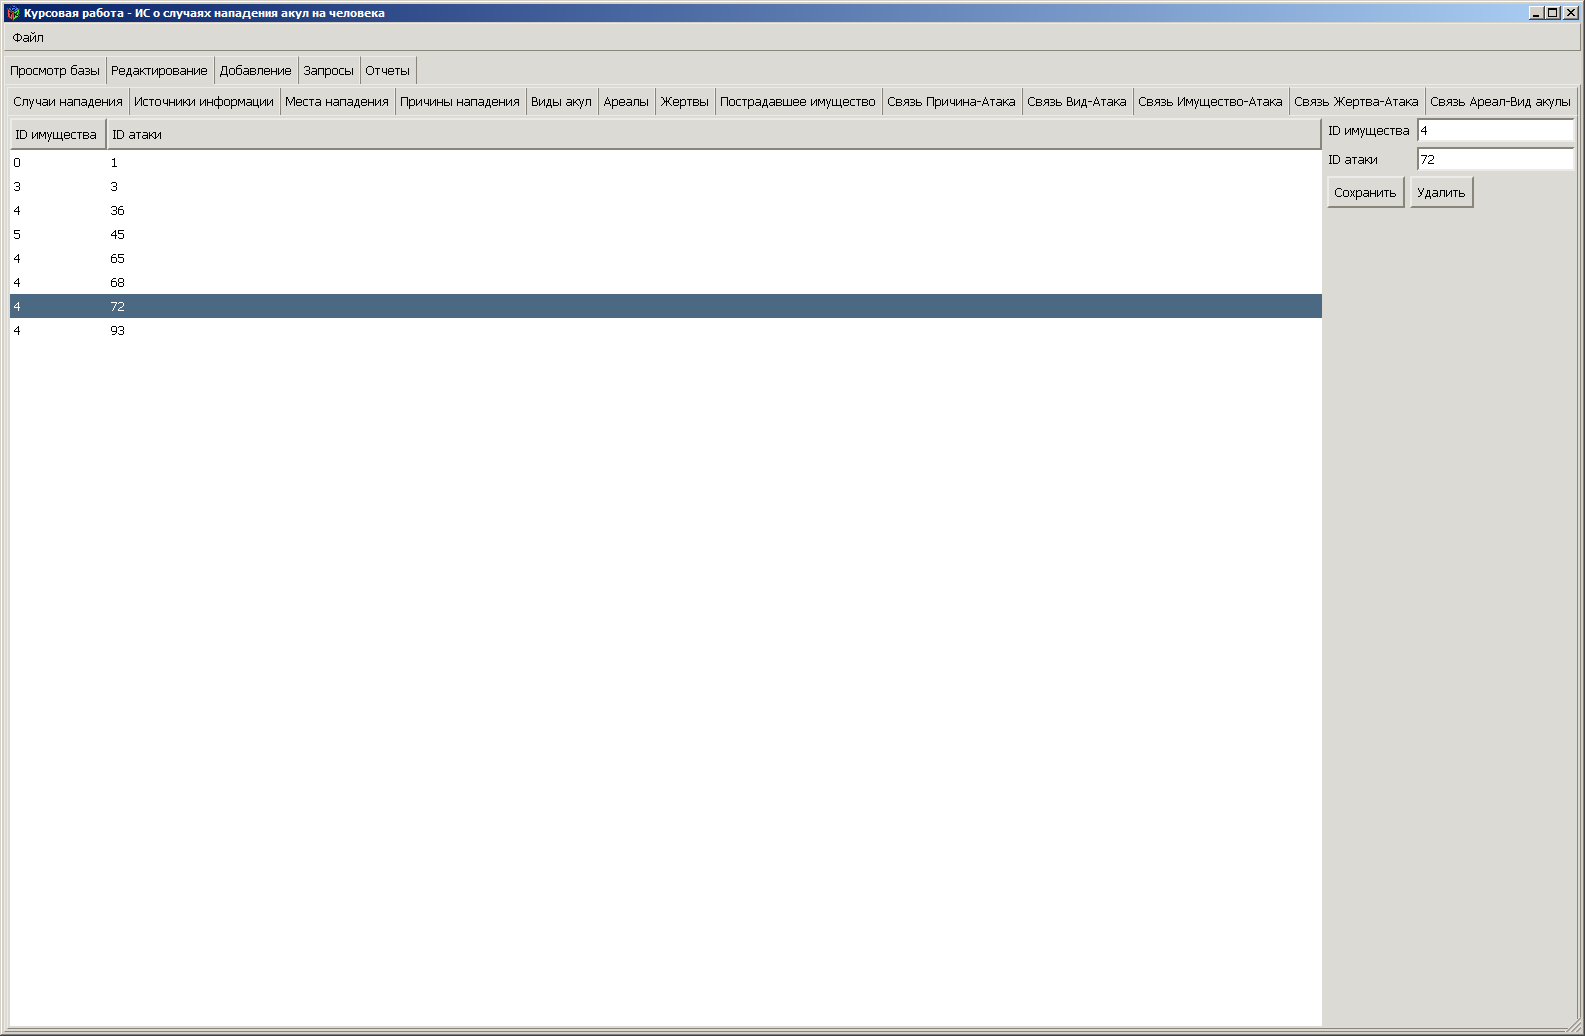
\includegraphics[width=\textwidth]{form24}
\caption{Форма <<Редактирование>>, таблица <<Связь Имущество-Атака>>}
\end{figure}

\begin{figure}[hb]
\centering
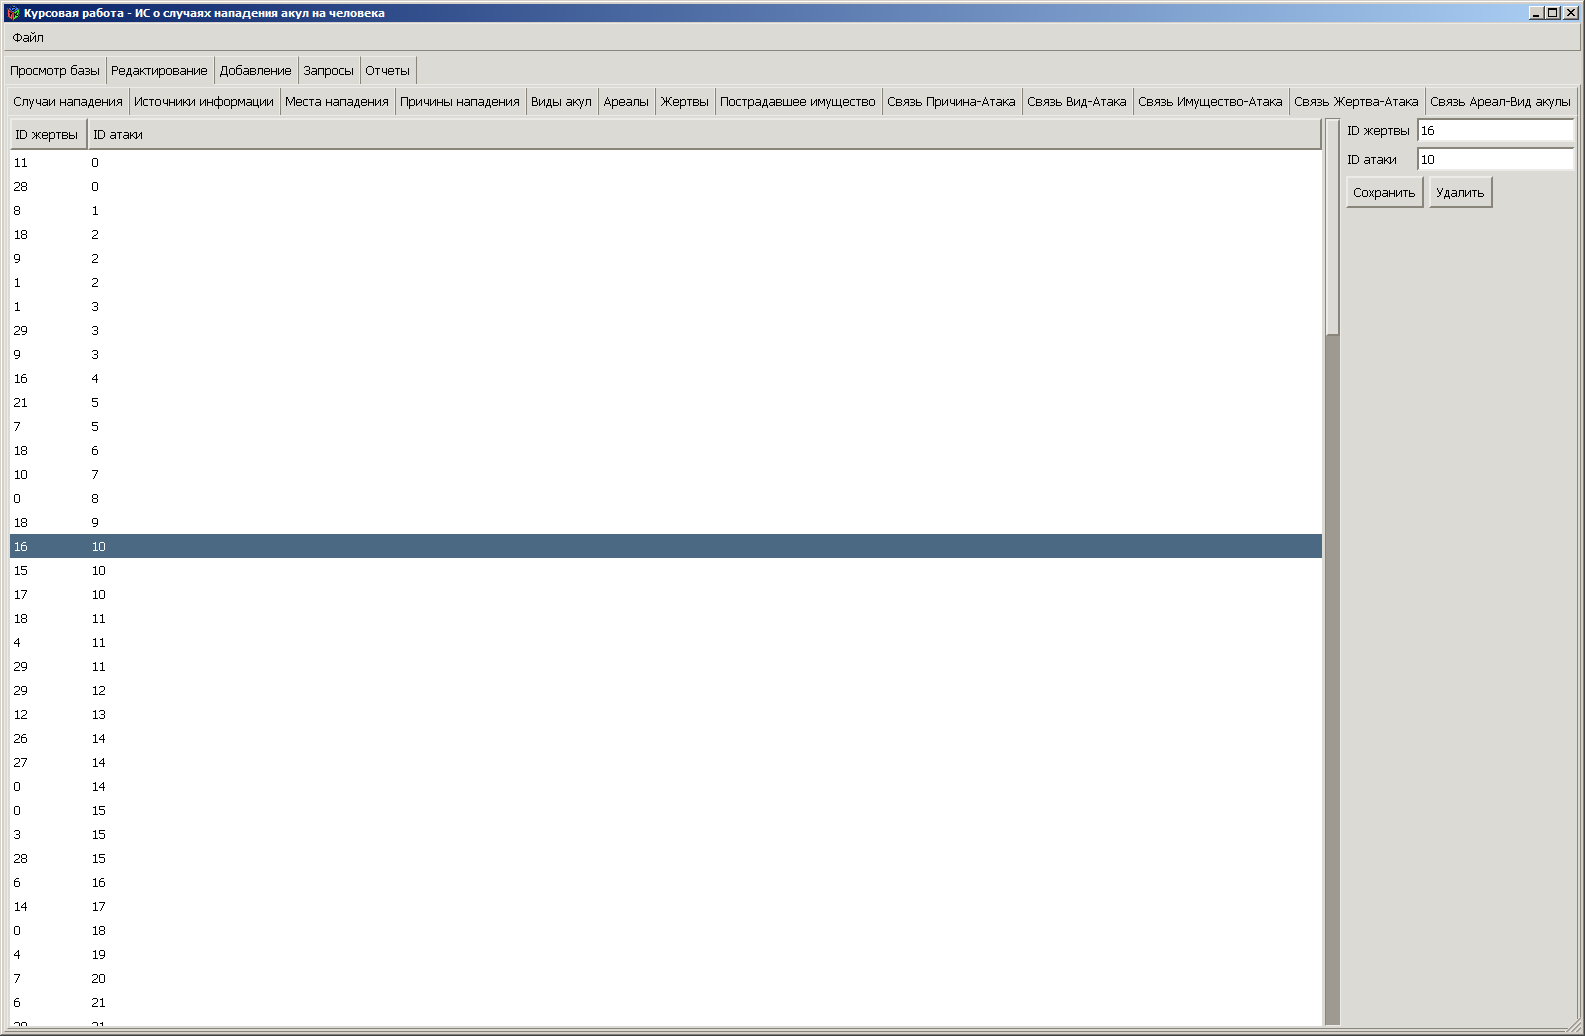
\includegraphics[width=\textwidth]{form25}
\caption{Форма <<Редактирование>>, таблица <<Связь Жертва-Атака>>}
\end{figure}

\begin{figure}[ht]
\centering
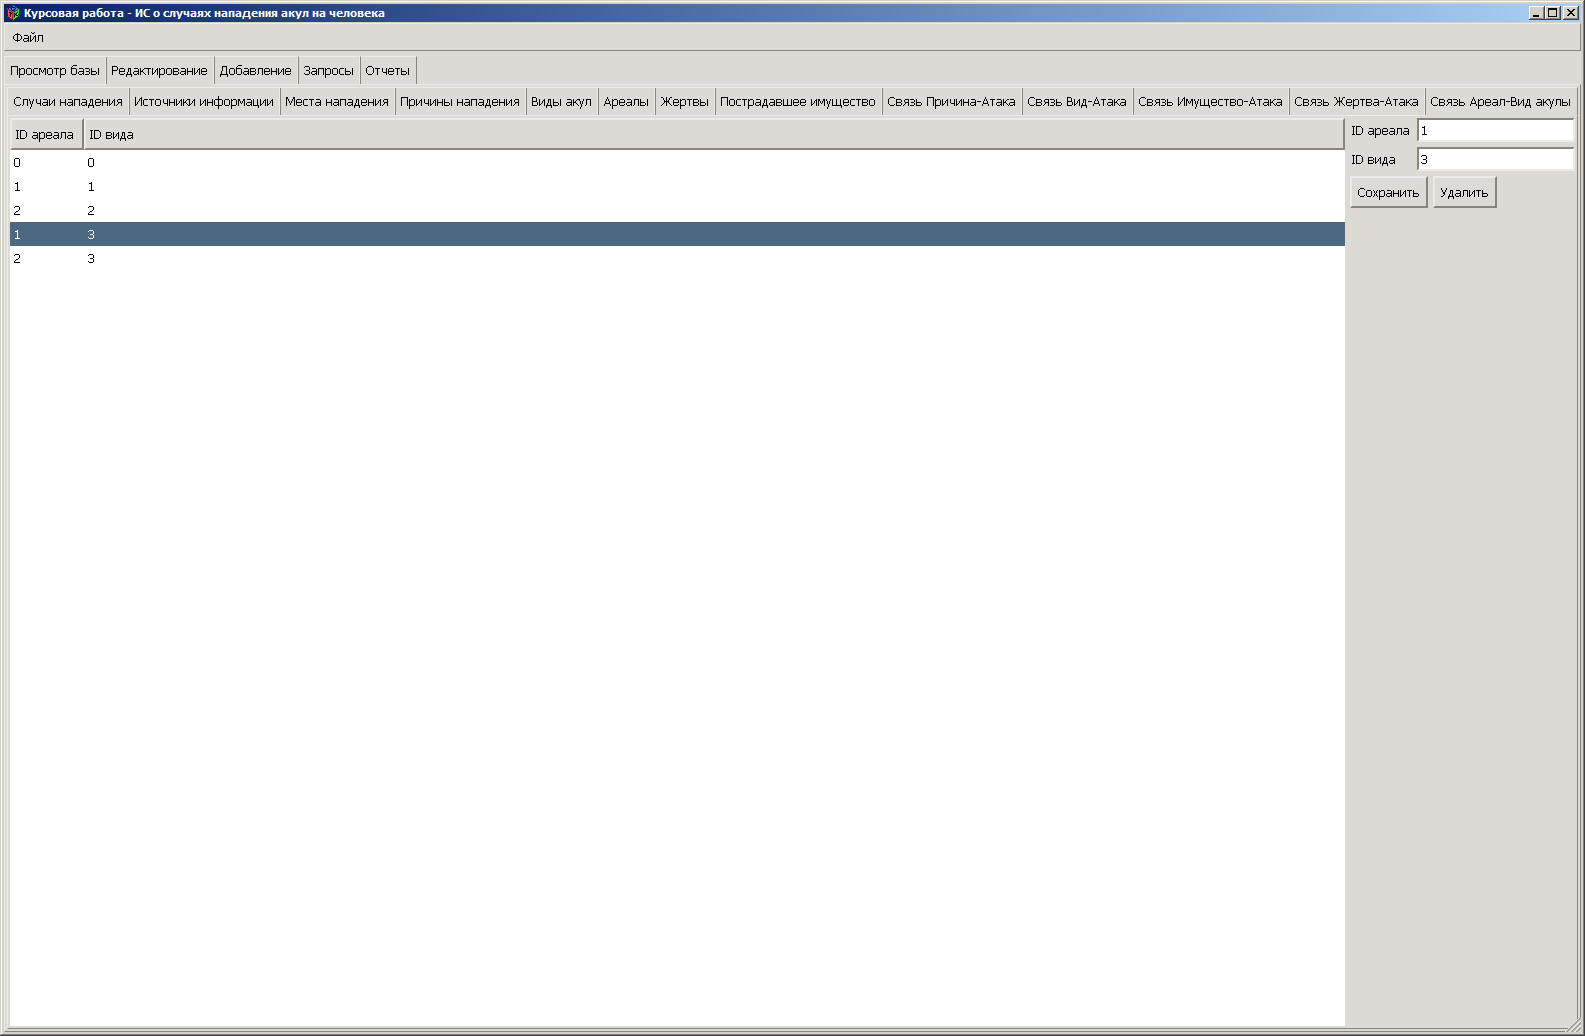
\includegraphics[width=\textwidth]{form26}
\caption{Форма <<Редактирование>>, таблица <<Связь Ареал-Вид акулы>>}
\end{figure}

\clearpage
\subsection{Формы добавления записей в таблицы}
\begin{figure}[ht]
\centering
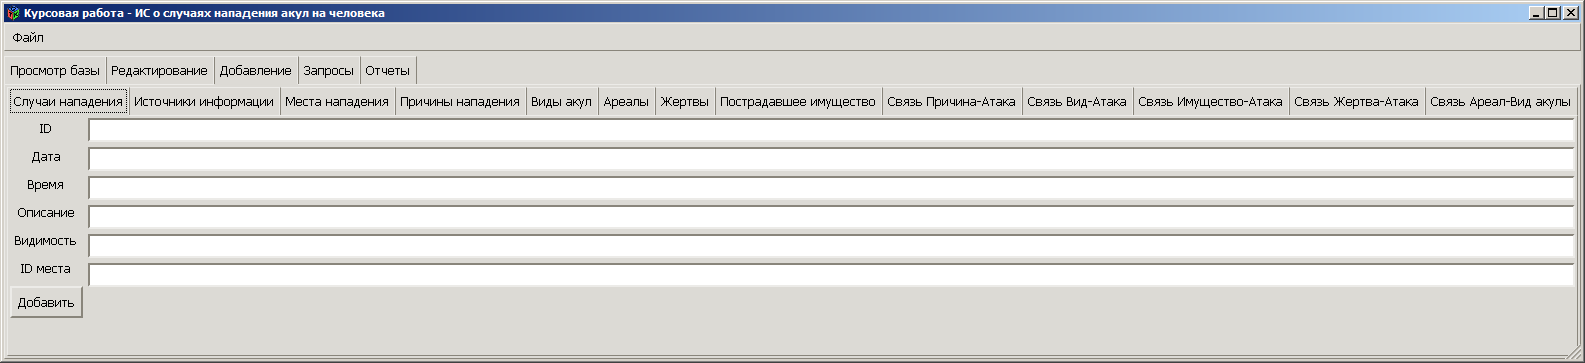
\includegraphics[width=\textwidth]{form27}
\caption{Форма <<Добавление>>, таблица <<Случаи нападения>>}
\end{figure}

\begin{figure}[hb]
\centering
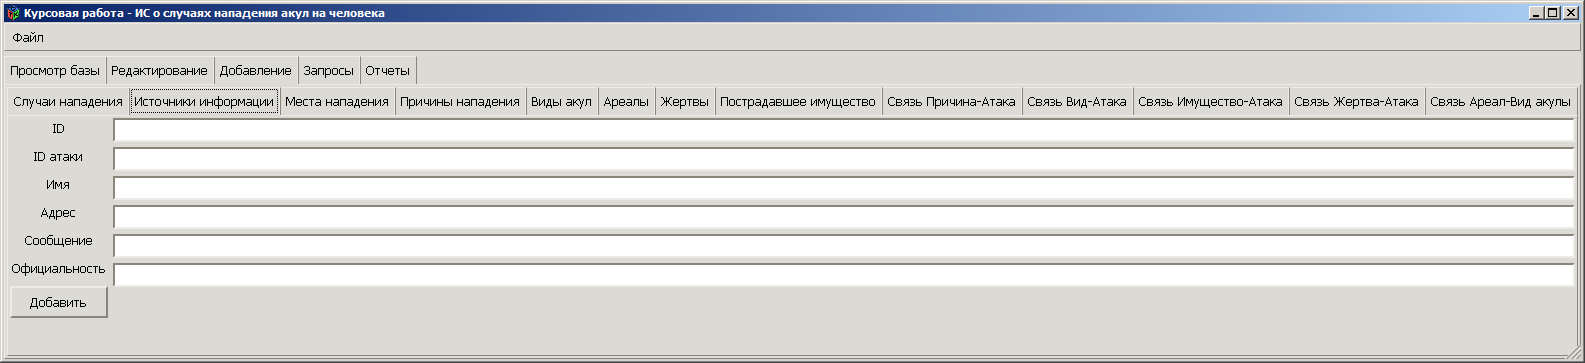
\includegraphics[width=\textwidth]{form28}
\caption{Форма <<Добавление>>, таблица <<Источники информации>>}
\end{figure}

\begin{figure}[ht]
\centering
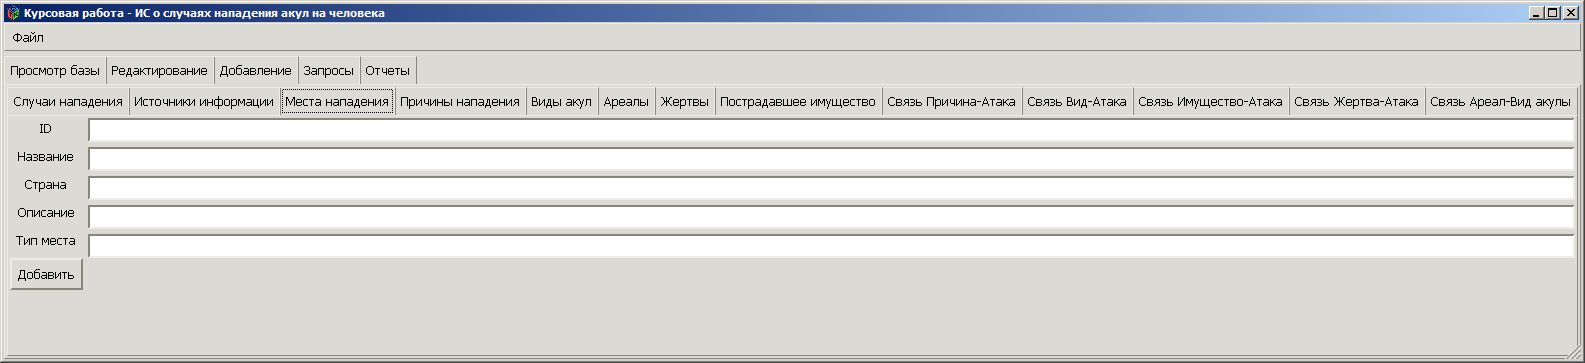
\includegraphics[width=\textwidth]{form29}
\caption{Форма <<Добавление>>, таблица <<Места нападения>>}
\end{figure}

\begin{figure}[hb]
\centering
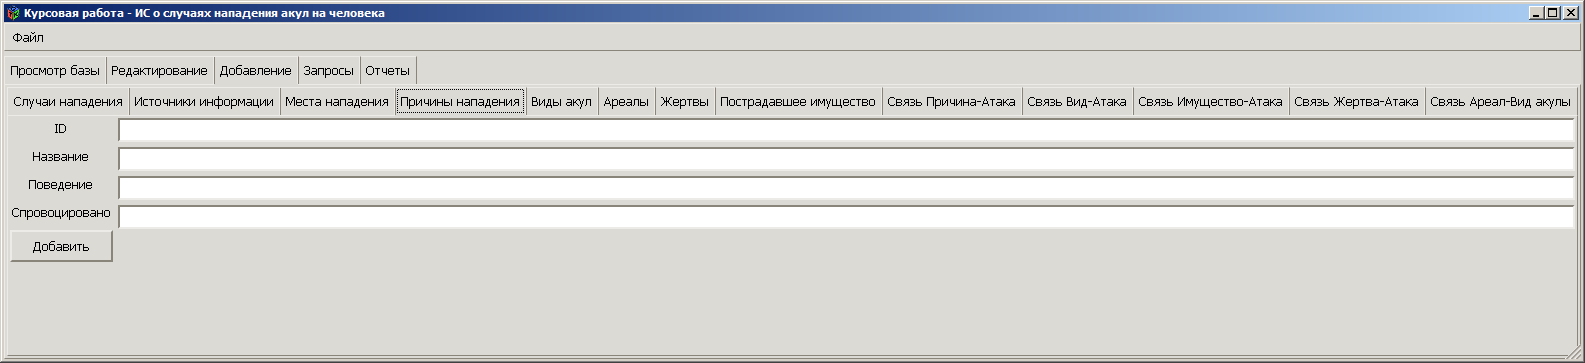
\includegraphics[width=\textwidth]{form30}
\caption{Форма <<Добавление>>, таблица <<Причины нападения>>}
\end{figure}

\begin{figure}[ht]
\centering
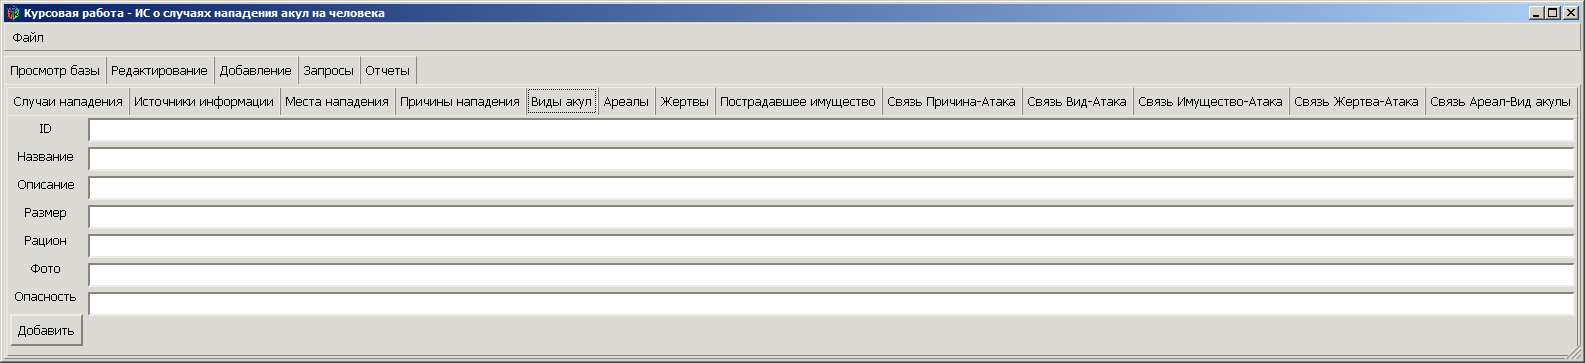
\includegraphics[width=\textwidth]{form31}
\caption{Форма <<Добавление>>, таблица <<Виды акул>>}
\end{figure}

\begin{figure}[hb]
\centering
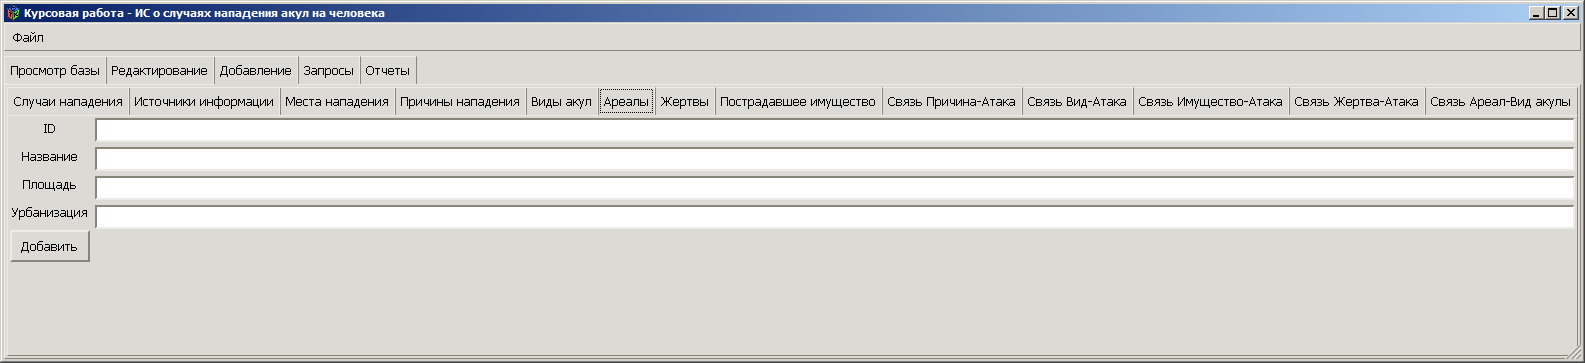
\includegraphics[width=\textwidth]{form32}
\caption{Форма <<Добавление>>, таблица <<Ареалы>>}
\end{figure}

\begin{figure}[ht]
\centering
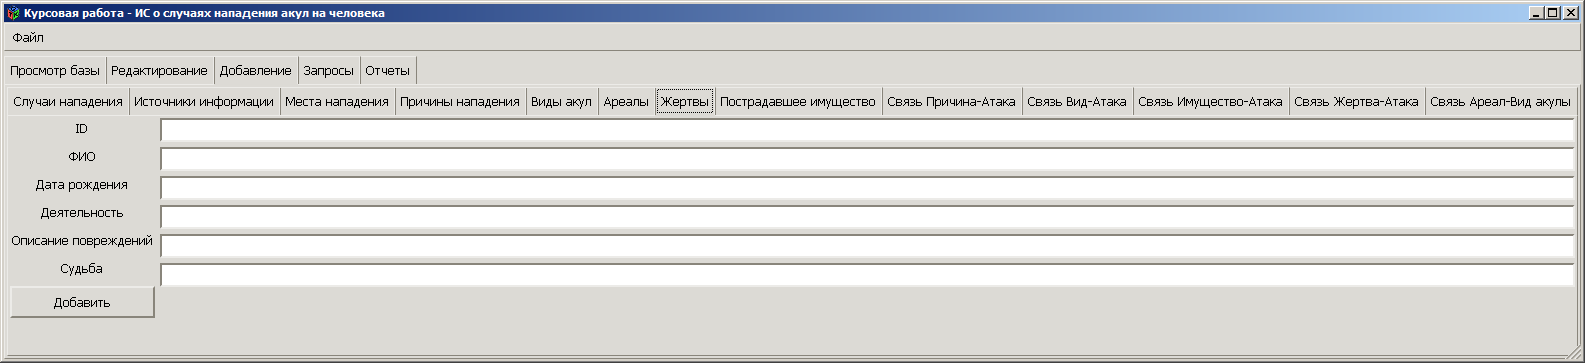
\includegraphics[width=\textwidth]{form33}
\caption{Форма <<Добавление>>, таблица <<Жертвы>>}
\end{figure}

\begin{figure}[hb]
\centering
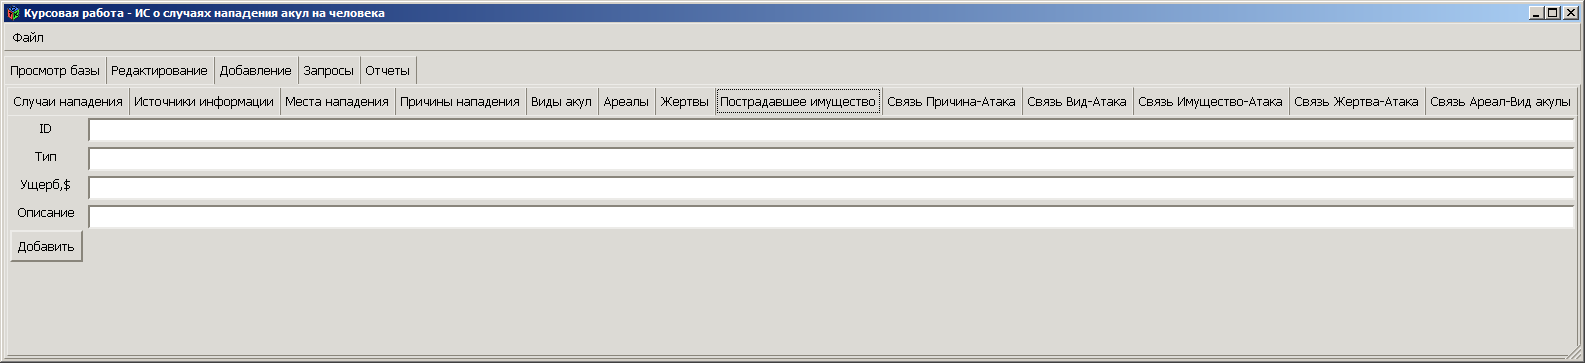
\includegraphics[width=\textwidth]{form34}
\caption{Форма <<Добавление>>, таблица <<Пострадавшее имущество>>}
\end{figure}

\begin{figure}[ht]
\centering
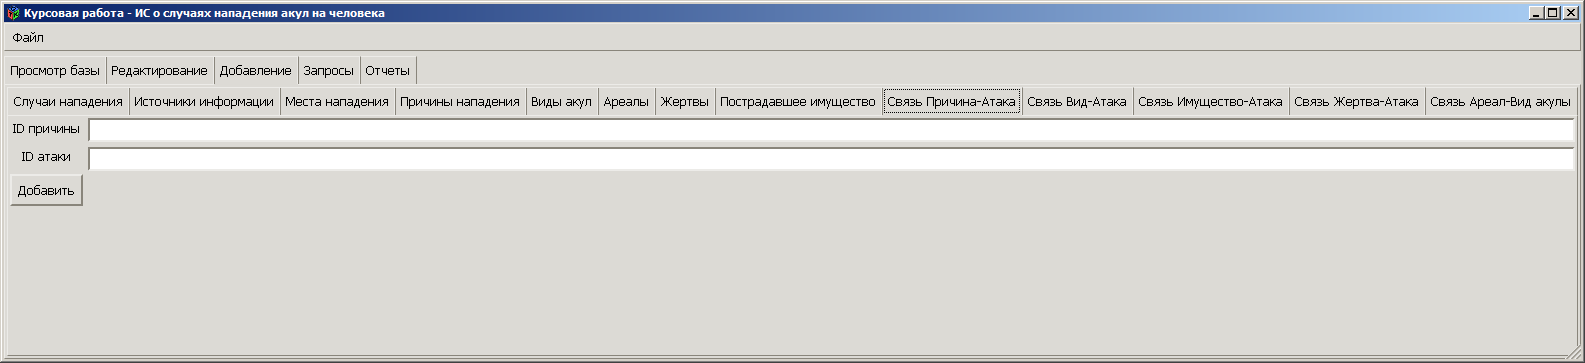
\includegraphics[width=\textwidth]{form35}
\caption{Форма <<Добавление>>, таблица <<Связь Причина-Атака>>}
\end{figure}

\begin{figure}[hb]
\centering
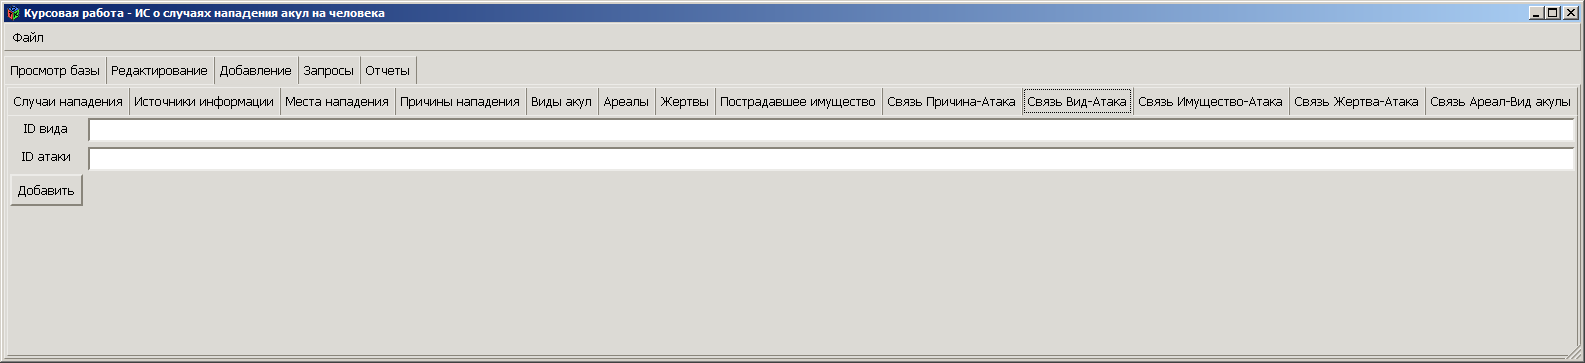
\includegraphics[width=\textwidth]{form36}
\caption{Форма <<Добавление>>, таблица <<Связь Вид-Атака>>}
\end{figure}

\begin{figure}[ht]
\centering
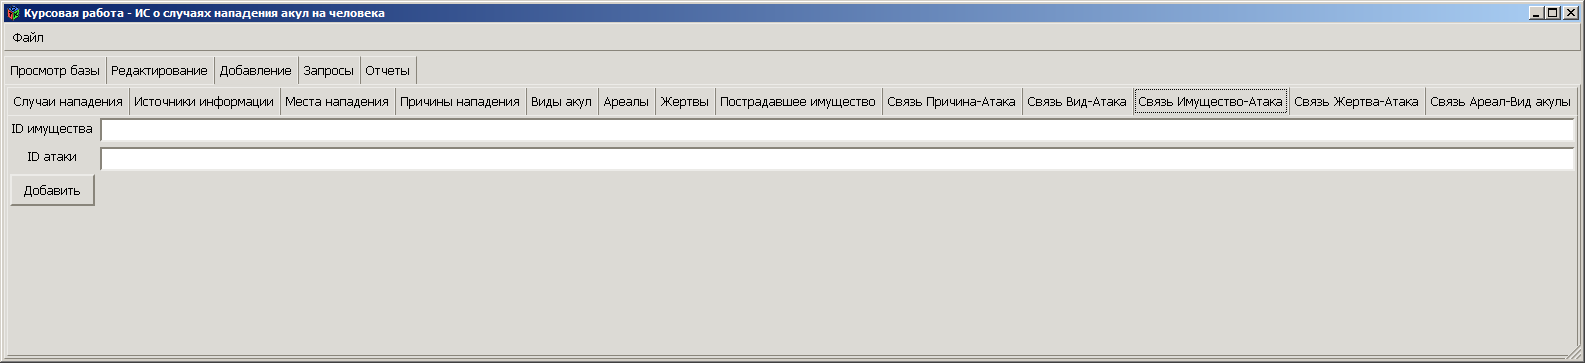
\includegraphics[width=\textwidth]{form37}
\caption{Форма <<Добавление>>, таблица <<Связь Имущество-Атака>>}
\end{figure}

\begin{figure}[hb]
\centering
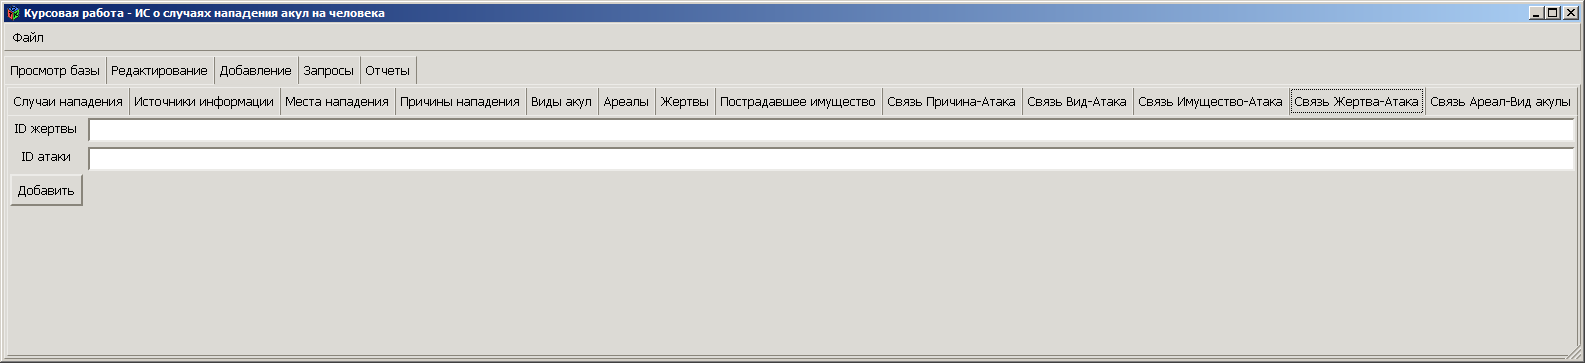
\includegraphics[width=\textwidth]{form38}
\caption{Форма <<Добавление>>, таблица <<Связь Жертва-Атака>>}
\end{figure}

\begin{figure}[ht]
\centering
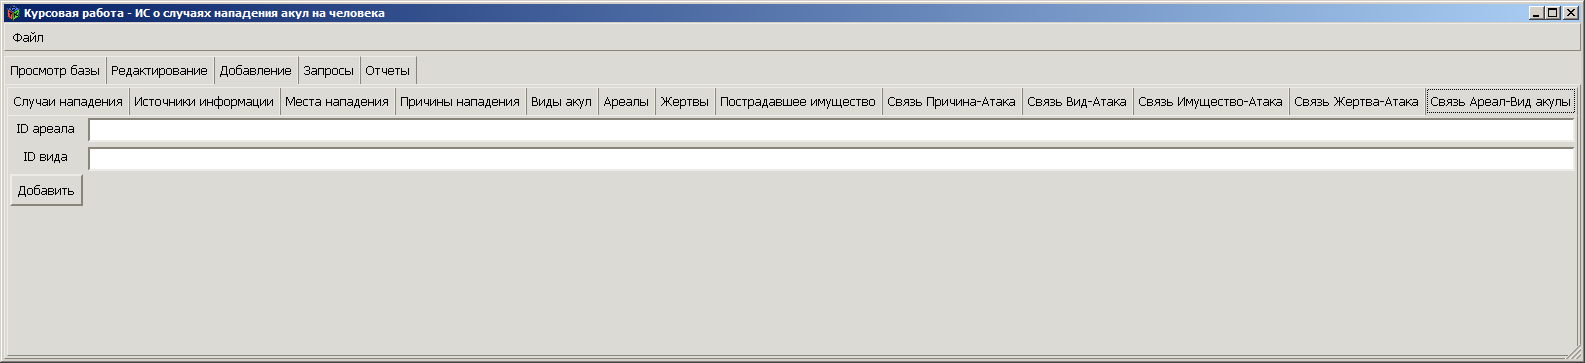
\includegraphics[width=\textwidth]{form39}
\caption{Форма <<Добавление>>, таблица <<Связь Ареал-Вид акулы>>}
\end{figure}

\clearpage
\subsection{Запросы}

\begin{figure}[ht]
\centering
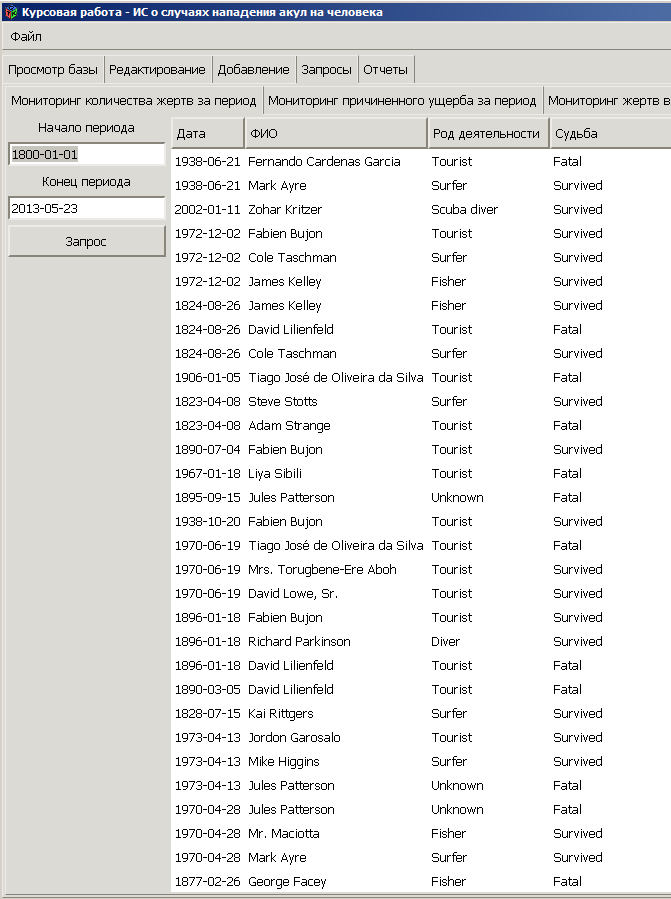
\includegraphics[scale=0.7]{query1}
\caption{Запрос <<Мониторинг количества жертв за период>>}
\end{figure}


\begin{figure}[ht]
\centering
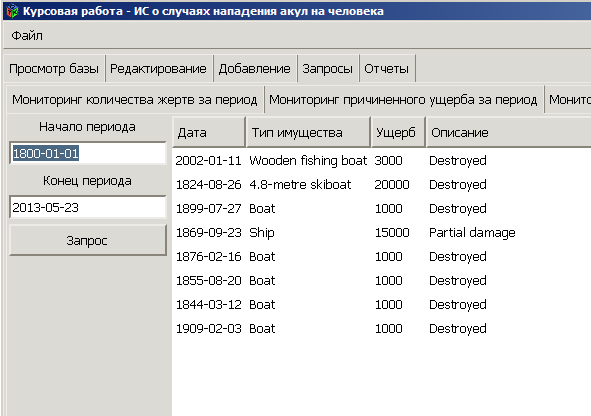
\includegraphics[scale=1.0]{query2}
\caption{Запрос <<Мониторинг причиненного ущерба за период>>}
\end{figure}

\begin{figure}[ht]
\centering
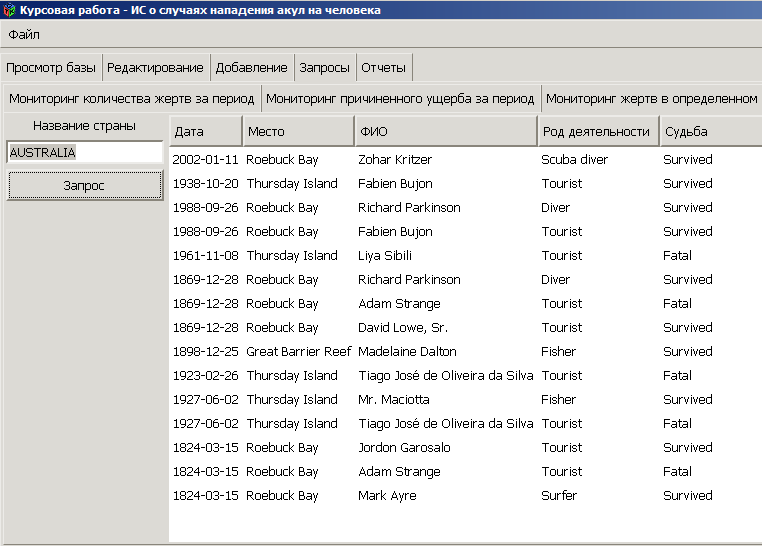
\includegraphics[scale=0.7]{query3}
\caption{Запрос <<Мониторинг жертв в определенном регионе>>}
\end{figure}

\begin{figure}[ht]
\centering
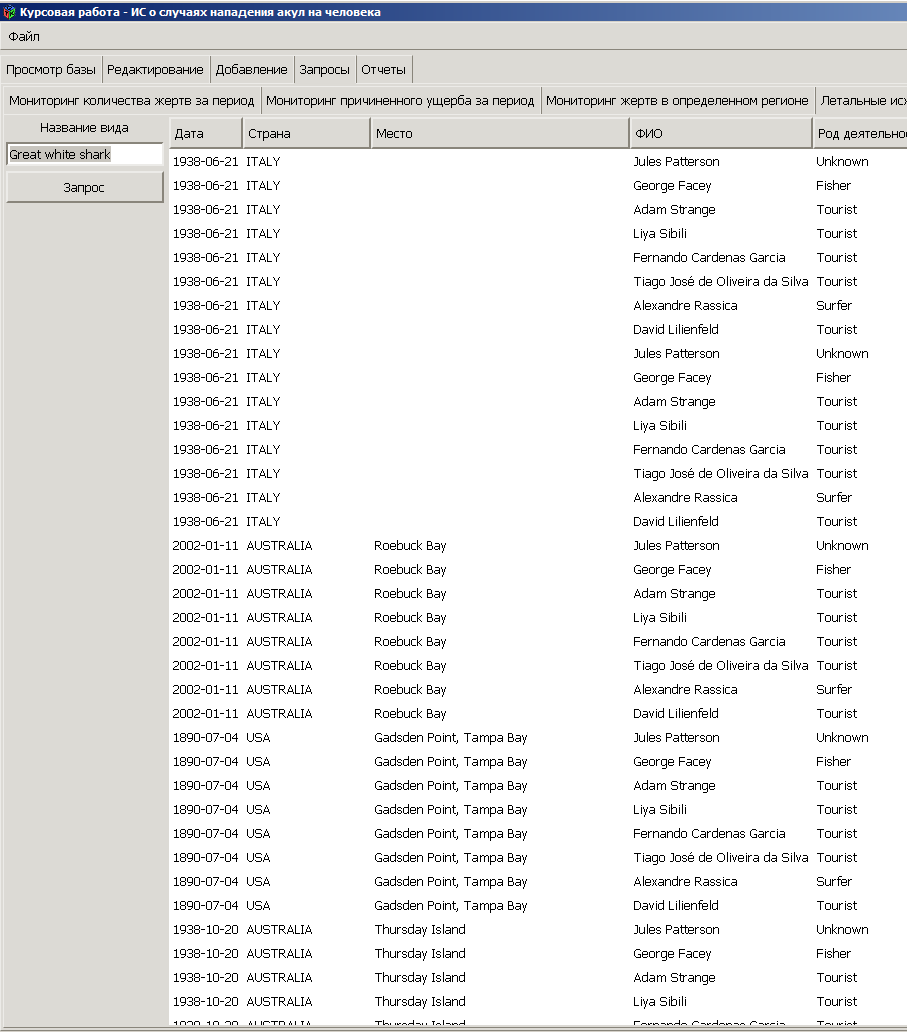
\includegraphics[scale=0.7]{query4}
\caption{Запрос <<Летальные исходы по виду акулы>>}
\end{figure}

\begin{figure}[ht]
\centering
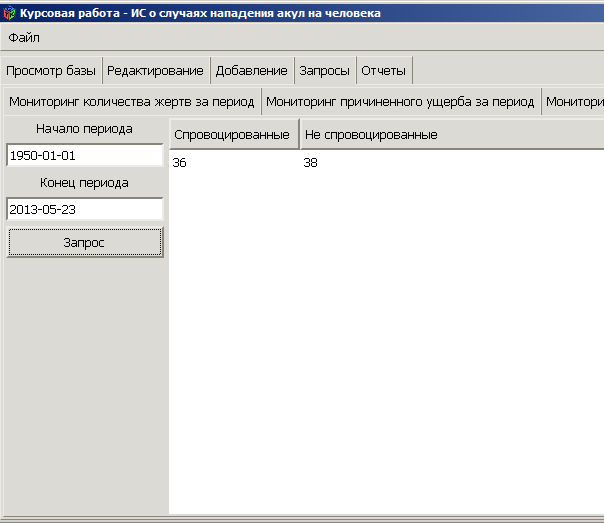
\includegraphics[scale=0.7]{query5}
\caption{Запрос <<Соотношение спровоцированных и не спровоцированных нападений за период>>}
\end{figure}

\end{document}
